\chapter{理想玻色系统}\label{ux7406ux60f3ux73bbux8272ux7cfbux7edf}
在延续第6.1节至第6.3节的内容之后，我们现在将深入研究一类系统的物理行为：在这些系统中，尽管分子间相互作用仍可忽略不计，但量子统计效应——即因粒子的不可区分性而产生的效应——却日益凸显其重要性。这意味着，系统的温度 \(T\) 和粒子密度 \(n\) 已不再符合以下准则：
\begin{equation}\tag{7.1.1}\label{eq:7.1.1}
n \lambda ^{3} \equiv \frac { n h ^{3} } { ( 2 \pi m k T ) ^{3 / 2} } \ll 1 ,
\end{equation}
其中 \(\lambda\{ \equiv h/(2\pi mkT)^{1/2}\}\) 是粒子的平均热波长或热德布罗意波长。事实上，量 \(n\lambda^{3}\) 也被证明是一个极为合适的参数，通过它，系统各项物理性质得以得到充分的表述。当 \(n\lambda^{3} \rightarrow 0\) 时，系统各项物理性质会平滑地过渡到其经典对应物。对于 \(n\lambda^{3}\) 为小值但又不为零的情形，系统相关各量可以按此参数展开为幂级数；从这些展开式中，我们得以一窥经典行为偏离的开端。当 \(n\lambda^{3}\) 变得接近于 1 时，系统的行为将与经典行为有显著差异，并呈现出明显的量子效应。在这样的条件下对系统进行研究，使我们直面一组在经典统计学中尚不为人知的现象。
显而易见，当系统处于相对较低的温度和/或具有相对较高的粒子密度时，其表现出量子行为的可能性更高。此外，粒子质量越小，量子效应就越显著。
如今，当 \(n\lambda^{3}\) 接近于 1 时，系统的行为不仅会与典型的经典行为出现显著偏差，还会受到构成该系统的粒子是遵循玻色-爱因斯坦统计还是费米-狄拉克统计的影响。在这种情况下，这两种系统的性质截然不同。在本章中，我们将研究属于第一类的系统；而在后续章节中，我们将探讨属于第二类的系统。
\section{理想玻色气体的热力学行为}\label{ux7406ux60f3ux73bbux8272ux6c14ux4f53ux7684ux70edux529bux5b66ux884cux4e3a}
在第6.1节和第6.2节中，我们得到了理想玻色气体的以下公式：
\begin{equation}\tag{7.1.2}\label{eq:7.1.2}
\frac { P V } { k T } \equiv \ln \mathcal { Q } = - \sum _ { \varepsilon } \ln ( 1 - z e ^{- \beta \varepsilon} )
\end{equation}
以及
\begin{equation}\tag{7.1.3}\label{eq:7.1.3}
N \equiv \sum _ { \varepsilon } \langle n _ { \varepsilon } \rangle = \sum _ { \varepsilon } \frac { 1 } { z ^{- 1} e ^{\beta \varepsilon} - 1 } ,
\end{equation}
其中 \(\beta = 1/kT\)，而 \(z\) 则是气体的逸度（fugacity），它与化学势 \(\mu\) 的关系由下式给出：
\begin{equation}\tag{7.1.4}\label{eq:7.1.4}
z \equiv \exp ( \mu / k T ) ;
\end{equation}
如前所述，对于任意 \(\varepsilon\)，\(z e^{-\beta\varepsilon} < 1\)。鉴于在大体积 \(V\) 条件下，单粒子态能谱几乎连续，因此可以将\autoref{eq:7.1.2}和\autoref{eq:7.1.3}右侧的求和替换为积分。在此过程中，我们利用了非相对论态密度 \(a(\varepsilon)\) 在给定能量 \(\varepsilon\) 附近的一般渐近表达式（2.4.7），即\(^{2}\)
\begin{equation}\tag{7.1.5}\label{eq:7.1.5}
a ( \varepsilon ) d \varepsilon = ( 2 \pi V / h ^{3} ) ( 2 m ) ^{3 / 2} \varepsilon ^{1 / 2} d \varepsilon .
\end{equation}
然而，我们注意到，将这一表达式代入我们的积分中，却无意间使能量水平 \(\varepsilon=0\) 的权重降为零。这种做法是错误的，因为在量子力学的处理中，我们必须为系统中的每一个非简并单粒子态赋予统计权重1。因此，在进行积分之前，最好先将这一特定状态从相关求和中剔除；关于这一（不同寻常）步骤的严格论证，请参见附录F。由此我们得到
\begin{equation}\tag{7.1.6}\label{eq:7.1.6}
\frac { P } { k T } = - \frac { 2 \pi } { h ^{3} } ( 2 m ) ^{3 / 2} \int _ { 0 } ^{\infty} \varepsilon ^{1 / 2} \ln ( 1 - z e ^{- \beta \varepsilon} ) d \varepsilon - \frac { 1 } { V } \ln ( 1 - z )
\end{equation}
并且
\begin{equation}\tag{7.1.7}\label{eq:7.1.7}
\frac { N } { V } = \frac { 2 \pi } { h ^{3} } ( 2 m ) ^{3 / 2} \int _ { 0 } ^{\infty} \frac { \varepsilon ^{1 / 2} d \varepsilon } { z ^{- 1} e ^{\beta \varepsilon} - 1 } + \frac { 1 } { V } \frac { z } { 1 - z } ;
\end{equation}
当然，这些积分的下限仍可取为0，因为\(\varepsilon=0\) 这一状态本身无论如何都不会对它们产生贡献。
在继续深入之前，先来谈谈\autoref{eq:7.1.6}和\autoref{eq:7.1.7}中最后几项的相对重要性。当 \(z \ll 1\) 时，这对应于与\ldots\ldots 相去不远的情形，
在经典极限下，这些项的阶数均为 \(1/N\)，因此可以忽略不计。然而，随着 \(z\) 增大并趋近于 1，\autoref{eq:7.1.7}中 \(z/(1-z)V\) 这一项——其值恒等于 \(N_0/V\)（其中 \(N_0\) 为基态 \(\varepsilon=0\) 中的粒子数）——很可能成为 \(N/V\) 的显著部分；当大量粒子汇聚到单一状态 \(\varepsilon=0\) 时，便会产生玻色-爱因斯坦凝聚现象。不过，由于 \(z/(1-z)=N_0\)，从而 \(z=N_0/(N_0+1)\)，\autoref{eq:7.1.6}中 \(-V^{-1}\ln(1-z)\) 这一项等于 \(V^{-1}\ln(N_0+1)\)，其值最多仅为 \(O(N^{-1}\ln N)\)；因此，无论 \(z\) 取何值，这一项都可忽略不计，故可舍去。
现在，对\autoref{eq:7.1.6}和\autoref{eq:7.1.7}作变量替换 \(\beta \varepsilon = x\)，即可得
\begin{equation}\tag{7.1.8}\label{eq:7.1.8}
\frac { P } { k T } = - \frac { 2 \pi ( 2 m k T ) ^{3 / 2} } { h ^{3} } \int _ { 0 } ^{\infty} x ^{1 / 2} \ln ( 1 - z e ^{- x} ) d x = \frac { 1 } { \lambda ^{3} } g _ { 5 / 2 } ( z )
\end{equation}
并且
\begin{equation}\tag{7.1.9}\label{eq:7.1.9}
\frac { N - N _ { 0 } } { V } = \frac { 2 \pi ( 2 m k T ) ^{3 / 2} } { h ^{3} } \int _ { 0 } ^{\infty} \frac { x ^{1 / 2} d x } { z ^{- 1} e ^{x} - 1 } = \frac { 1 } { \lambda ^{3} } g _ { 3 / 2 } ( z ) ,
\end{equation}
其中
\begin{equation}\tag{7.1.10}\label{eq:7.1.10}
\lambda = h / ( 2 \pi m k T ) ^{1 / 2} ,
\end{equation}
而 \(g_{\nu}(z)\) 是由附录D所定义的玻色-爱因斯坦函数，
\begin{equation}\tag{7.1.11}\label{eq:7.1.11}
g _ { \nu } ( z ) = \frac { 1 } { \Gamma ( \nu ) } \int _ { 0 } ^{\infty} \frac { x ^{\nu - 1} d x } { z ^{- 1} e ^{x} - 1 } = z + \frac { z ^{2} } { 2 ^{\nu} } + \frac { z ^{3} } { 3 ^{\nu} } + \cdots ;
\end{equation}
请注意，要将\autoref{eq:7.1.8}表示为 \(g_{5/2}(z)\) 函数的形式，我们首先进行了分部积分。\autoref{eq:7.1.8}和\autoref{eq:7.1.9}是我们基本的结论；通过消去 \(z\)，这两式将为我们提供系统的状态方程。
该系统的内能由以下公式给出
\begin{equation}\tag{7.1.12}\label{eq:7.1.12}
\begin{array}{rlr} & { } & { U \equiv - \left( \frac { \partial } { \partial \beta } \ln \mathcal { Q } \right) _ { z , V } = k T ^{2} \left\{ \frac { \partial } { \partial T } \left( \frac { P V } { k T } \right) \right\} _ { z , V } } \\& { } & { = k T ^{2} V \, g _ { 5 / 2 } ( z ) \left\{ \frac { d } { d T } \left( \frac { 1 } { \lambda ^{3} } \right) \right\} = \frac { 3 } { 2 } k T \frac { V } { \lambda ^{3} } g _ { 5 / 2 } ( z ) ; } \end{array}
\end{equation}
此处已利用了\autoref{eq:7.1.8}以及\(\lambda \propto T^{-1/2}\)这一事实。因此，从广义上讲，我们的系统满足以下关系：
\begin{equation}\tag{7.1.13}\label{eq:7.1.13}
P = \frac { 2 } { 3 } ( U / V ) .
\end{equation}
对于小值的\(z\)，我们可以利用展开式\autoref{eq:7.1.11}；同时，我们也可以将\(N_0\)与\(N\)相比较，将其视为可忽略不计。随后，我们可以在\autoref{eq:7.1.8}和\autoref{eq:7.1.9}之间消去\(z\)，从而得到
首先对\autoref{eq:7.1.9}中的级数进行求逆变换，以获得\(z\)的幂级数展开式，然后将该展开式代入\autoref{eq:7.1.8}中所出现的级数。由此，状态方程的形式便演变为维里展开式，
\begin{equation}\tag{7.1.14}\label{eq:7.1.14}
\frac { P V } { N k T } = \sum _ { l = 1 } ^{\infty} a _ { l } \left( \frac { \lambda ^{3} } { \nu } \right) ^{l - 1} ,
\end{equation}
其中\(\nu(\equiv 1/n)\)为每粒子的体积；这些系数\(a_{l}\)，即系统的维里系数，最终被证明为
\begin{equation}\tag{7.1.15}\label{eq:7.1.15}
\left. \begin{array}{l} { { a _ { 1 } = 1 , } } \\{ { a _ { 2 } = - \frac { 1 } { 4 \sqrt { 2 } } = - 0 . 17 67 8 , } } \\{ { a _ { 3 } = - \left( \frac { 2 } { 9 \sqrt { 3 } } - \frac { 1 } { 8 } \right) = - 0 . 00 33 0 , } } \\{ { a _ { 4 } = - \left( \frac { 3 } { 32 } + \frac { 5 } { 32 \sqrt { 2 } } - \frac { 1 } { 2 \sqrt { 6 } } \right) = - 0 . 00 01 1 , } } \end{array} \right\}
\end{equation}
以此类推。对于气体的比热，我们得到
\begin{equation}\tag{7.1.16}\label{eq:7.1.16}
\begin{array}{rl} & { \frac { C _ { V } } { N k } \equiv \frac { 1 } { N k } \left( \frac { \partial U } { \partial T } \right) _ { N , V } = \frac { 3 } { 2 } \left\{ \frac { \partial } { \partial T } \left( \frac { P V } { N k } \right) \right\} _ { \nu } } \\& {  = \frac { 3 } { 2 } \sum _ { l = 1 } ^{\infty} \frac { 5 - 3 l } { 2 } a _ { l } \left( \frac { \lambda ^{3} } { \nu } \right) ^{l - 1} } \\& {  = \frac { 3 } { 2 } \left[ 1 + 0 . 08 84 \left( \frac { \lambda ^{3} } { \nu } \right) + 0 . 00 66 \left( \frac { \lambda ^{3} } { \nu } \right) ^{2} + 0 . 00 04 \left( \frac { \lambda ^{3} } { \nu } \right) ^{3} + \cdots \right] . } \end{array}
\end{equation}
当\(T \to \infty\)（进而\(\lambda \to 0\)）时，气体的压力和比热分别趋近于其经典值，即\(nkT\)和\(\frac{3}{2}Nk\)。我们还注意到，在有限但较高的温度下，气体的比热会高于其极限值；换言之，\((C_V, T)\)曲线在高温区间呈现出负斜率。另一方面，当\(T \to 0\)时，比热必然趋近于零。因此，它必须在某处穿过一个最大值。正如后续所见，这一最大值本质上是一种尖峰，出现在临界温度\(T_c\)处；在该温度下，比热的导数被发现存在不连续性（详见本节后文图~7.4）。
随着系统温度的降低（参数\(\lambda^{3}/\nu\)的值随之增大），诸如\autoref{eq:7.1.14}和\autoref{eq:7.1.16}之类的展开式便不再适用。此时，我们只能沿用\autoref{eq:7.1.8}、\autoref{eq:7.1.9}和\autoref{eq:7.1.11}等公式。而\(z\)的精确值现在可通过\autoref{eq:7.1.9}求得，该式可重写为
\begin{equation}\tag{7.1.17}\label{eq:7.1.17}
N _ { e } = V \frac { ( 2 \pi m k T ) ^{3 / 2} } { h ^{3} } g _ { 3 / 2 } ( z ) ,
\end{equation}
其中\(N_{e}\)为激发态中的粒子数（\(\varepsilon \neq 0\)）；当然，除非\(z\)极度接近于1，否则\(N_{e} \simeq N\)。\(^{3}\) 显而易见，在\(0 \leq z \leq 1\) 的范围内，函数\(g_{3/2}(z)\)随\(z\)单调递增且有界，其最大值为
\begin{equation}\tag{7.1.18}\label{eq:7.1.18}
g _ { 3 / 2 } ( 1 ) = 1 + \frac { 1 } { 2 ^{3 / 2} } + \frac { 1 } { 3 ^{3 / 2} } + \cdots \equiv \zeta \left( \frac { 3 } { 2 } \right) \simeq 2 . 61 2 ;
\end{equation}
参见附录D中的式（D.5）。因此，对于所有感兴趣的\(z\)，
\begin{equation}\tag{7.1.19}\label{eq:7.1.19}
g _ { 3 / 2 } ( z ) \leq \zeta \left( \frac { 3 } { 2 } \right) .
\end{equation}
因此，对于给定的\(V\)和\(T\)，所有激发态中粒子的总（平衡）数量也受到限制，即
\begin{equation}\tag{7.1.20}\label{eq:7.1.20}
N _ { e } \leq V \frac { ( 2 \pi \, m k T ) ^{3 / 2} } { h ^{3} } \zeta \left( \frac { 3 } { 2 } \right) .
\end{equation}
目前，只要系统中粒子的实际数量低于这一临界值，一切就都很好；实际上，系统中的几乎所有粒子都分布在激发态上，而\(z\)的精确数值则由\autoref{eq:7.1.17}决定，且有\(N_{e} \simeq N\)。然而，如果粒子的实际数量超过这一临界值，那么激发态自然会尽可能多地容纳这些粒子，即
\begin{equation}\tag{7.1.21}\label{eq:7.1.21}
N _ { e } = V \frac { ( 2 \pi m k T ) ^{3 / 2} } { h ^{3} } \zeta \left( \frac { 3 } { 2 } \right) ,
\end{equation}
而其余的粒子将被大量推向基态\(\varepsilon=0\)（在任何情况下，该基态的容量基本上都是无限的）：
\begin{equation}\tag{7.1.22}\label{eq:7.1.22}
N _ { 0 } = N - \left\{ V \frac { ( 2 \pi \, m k T ) ^{3 / 2} } { h ^{3} } \zeta \left( \frac { 3 } { 2 } \right) \right\} .
\end{equation}
\(z\)的精确数值现在由以下公式决定：
\begin{equation}\tag{7.1.23}\label{eq:7.1.23}
z = \frac { N _ { 0 } } { N _ { 0 } + 1 } \simeq 1 - \frac { 1 } { N _ { 0 } }
\end{equation}
在实际应用中，这一数值几乎等于1。这种奇特的现象——即宏观尺度上的大量粒子聚集于单一量子态（\(\varepsilon=0\)）——通常被称为玻色-爱因斯坦凝聚现象。从某种意义上说，这一现象与我们熟悉的蒸汽凝结成液体的过程颇为相似，而后者发生在普通的物理空间中。不过，从概念上讲，这两种过程却大不相同。首先，玻色-爱因斯坦凝聚现象纯粹是
源于量子力学的原理（即使在不存在分子间作用力的情况下也会发生）；其次，它最多只发生在动量空间中，而非坐标空间中。\(^{4}\)
玻色-爱因斯坦凝聚开始的条件是
\begin{equation}\tag{7.1.24}\label{eq:7.1.24}
N > V T ^{3 / 2} \frac { ( 2 \pi \, m k ) ^{3 / 2} } { h ^{3} } \zeta \left( \frac { 3 } { 2 } \right)
\end{equation}
或者，如果我们保持\(N\)和\(V\)不变，而改变\(T\)，
\begin{equation}\tag{7.1.25}\label{eq:7.1.25}
T < T _ { c } = \frac { h ^{2} } { 2 \pi m k } \left\{ \frac { N } { V _ { \zeta } \left( \frac { 3 } { 2 } \right) } \right\} ^{2 / 3} ;
\end{equation}
在此，\(T_{c}\)代表一个特征温度，该温度取决于系统的粒子质量\(m\)以及粒子密度\(N/V\)。因此，在\(T < T_{c}\)时，我们可以将系统视为两种"相"的混合体：
\begin{enumerate}
\def\labelenumi{(\roman{enumi})}
\item
  正常相，由\(N_{e} \{= N(T/T_{c})^{3/2}\}\)个粒子组成，这些粒子分布在激发态（\(\varepsilon \neq 0\)）中；并且
\item
  凝聚相，由\(N_{0} \{=(N-N_{e})\}\)个粒子构成，这些粒子聚集在基态（\(\varepsilon = 0\)）中。
\end{enumerate}
图~7.1展示了互补分数（\(N_{e}/N\)）和\((N_{0}/N)\)随\(T\)变化的规律。当\(T > T_{c}\)时，我们仅能见到正常相；基态中的粒子数，即\(z/(1-z)\)，仅为\(O(1)\)，与总粒子数\(N\)相比，这一数值几乎可以忽略不计。显然，当\(T = T_{c}\)时，情况变得极为特殊。稍后我们将提及，当\(T\)从下方逐渐接近\(T_{c}\)时，凝聚相的比例将按如下方式消失：
\begin{equation}\tag{7.1.26}\label{eq:7.1.26}
\frac { N _ { 0 } } { N } = 1 - \left( \frac { T } { T _ { c } } \right) ^{3 / 2} \approx \frac { 3 } { 2 } \frac { T _ { c } - T } { T _ { c } } .
\end{equation}
在此，了解\(z\)随\(T\)的变化规律也颇具意义。不过，将\(z\)与\((\nu/\lambda^3)\)的变化关系加以考虑要简单得多，而后者与\(T^{3/2}\)成正比。在\(0 \leq (\nu/\lambda^3) \leq (2.612)^{-1}\) 的范围内——即对应于\(0 \leq T \leq T_c\)——参数\(z\)近似为1；详见\autoref{eq:7.1.23}。当\((\nu/\lambda^3) > (2.612)^{-1}\) 时，\(z < 1\)，其值由以下关系决定：
\begin{equation}\tag{7.1.27}\label{eq:7.1.27}
g _ { 3 / 2 } ( z ) = ( \lambda ^{3} / v ) < 2 . 61 2 ;
\end{equation}
当然，这一现象在坐标空间中所引发的效应同样引人遐想。它为超流态的出现奠定了基础——这一量子现象将在第7.6节中进行详细讨论。
关于玻色-爱因斯坦凝聚的起始过程，可参阅兰兹伯格（1954b）的著作。该书还尝试对此前发表的大量相关研究成果进行了系统梳理与整合。更为近期的研究成果包括格林斯蓬与帕特里亚（1974年）、帕特里亚（1983年）以及附录F。
一个等价的关系是：\(g_{3/2}(z)/g_{3/2}(1)=(T_{c}/T)^{3/2}<1\)。
该压力与\(T^{5/2}\)成正比，并且与\(\nu\)无关——这意味着其压缩性趋于无穷大。在转变点处，压力的数值为
\begin{equation}\tag{7.1.28}\label{eq:7.1.28}
P ( T _ { c } ) = \left( \frac { 2 \pi \, m } { h ^{2} } \right) ^{3 / 2} ( k T _ { c } ) ^{5 / 2} \zeta \left( \frac { 5 } { 2 } \right) ;
\end{equation}
式（6.2.12）给出了理想经典气体的公式：\(\ln\mathcal{Q}=zV/\lambda^{3}\)。据此，\(N\equiv z(\partial\ln\mathcal{Q}/\partial z)=z(V/\lambda^{3})\)，从而得出\(z=(\lambda^{3}/v)\)。
借助\autoref{eq:7.1.25}，可以将其写为
\begin{equation}\tag{7.1.29}\label{eq:7.1.29}
P ( T _ { c } ) = \frac { \zeta \left( \frac { 5 } { 2 } \right) } { \zeta \left( \frac { 3 } { 2 } \right) } \left( \frac { N } { V } k T _ { c } \right) \simeq 0 . 51 34 \left( \frac { N } { V } k T _ { c } \right) .
\end{equation}
因此，在转变温度\(T_{c}\)下，理想玻色气体粒子所施加的压力约为等效玻尔兹曼气体粒子所施加压力的一半。⁸ 对于\(T > T_{c}\)，压力由以下公式给出：
\begin{equation}\tag{7.1.30}\label{eq:7.1.30}
P = \frac { N } { V } k T \frac { g _ { 5 / 2 } ( z ) } { g _ { 3 / 2 } ( z ) } ,
\end{equation}
其中\(z(T)\)由隐含关系决定
\begin{equation}\tag{7.1.31}\label{eq:7.1.31}
g _ { 3 / 2 } ( z ) = \frac { \lambda ^{3} } { \nu } = \frac { N } { V } \frac { h ^{3} } { ( 2 \pi m k T ) ^{3 / 2} } .
\end{equation}
除非\(T\)极高，否则压力\(P\)无法用更简单的形式来表示；当然，在\(T \gg T_{c}\)时，可以使用维里展开式\autoref{eq:7.1.14}。随着\(T\)趋近于无穷大，压力会接近经典值\(NkT/V\)。所有这些特征均在图~7.3中得到展示。图中的相变线对应于\autoref{eq:7.1.28}。实际的\((P, T)\)曲线从\(T=0\)一直延伸至\(T=T_{c}\)，随后偏离该线，并逐渐趋于经典极限。值得注意的是，相变线右侧的区域仅属于正常相，而该线本身则属于混合相；而左侧的区域对系统而言是不可达的。
鉴于气体的内能与其压力之间存在直接关系，如\autoref{eq:7.1.13}所示，图~7.3同样清晰地展示了\(U\)随\(T\)的变化规律（当然，在\(\nu\)保持不变的情况下）。因此，其斜率应被视为衡量气体比热容\(C_V(T)\)的指标。我们很容易发现，当温度较低时，比热容几乎为零；随着温度升高，比热容逐渐增加，直至在\(T = T_c\)时达到最大值；此后，比热容开始下降，并逐渐趋于恒定的经典值。从解析角度出发，在\(T \leq T_c\)时，我们可得{[}参见\autoref{eq:7.1.16}和\autoref{eq:7.1.28}{]}
\begin{equation}\tag{7.1.32}\label{eq:7.1.32}
\frac { C _ { V } } { N k } = \frac { 3 } { 2 } \frac { V } { N } \zeta \left( \frac { 5 } { 2 } \right) \frac { d } { d T } \left( \frac { T } { \lambda ^{3} } \right) = \frac { 15 } { 4 } \zeta \left( \frac { 5 } { 2 } \right) \frac { \nu } { \lambda ^{3} } ,
\end{equation}
实际上，对于所有\(T \leq T_{c}\)，我们都可以写成
\begin{equation}\tag{7.1.33}\label{eq:7.1.33}
P ( T ) = P ( T _ { c } ) \cdot ( T / T _ { c } ) ^{5 / 2} \simeq 0 . 51 34 ( N _ { e } k T / V ) .
\end{equation}
我们推断，虽然凝聚态中的粒子完全不产生压力，但处于激发态的粒子的效力却大约只有玻尔兹曼情形下的一半。
该值明显高于经典值1.5。对于\(T > T_{c}\)，我们得到了一个隐含的公式。首先，
\begin{equation}\tag{7.1.34}\label{eq:7.1.34}
\frac { C _ { V } } { N k } = \left[ \frac { \partial } { \partial T } \left( \frac { 3 } { 2 } \, T \frac { g _ { 5 / 2 } ( z ) } { g _ { 3 / 2 } ( z ) } \right) \right] _ { \nu } ;
\end{equation}
参见\autoref{eq:7.1.12}和\autoref{eq:7.1.27}。要进行求导运算，我们需要知道\((\partial z/\partial T)_v\)；这一结果可通过\autoref{eq:7.1.27}结合附录D中的递推关系（D.10）来获得。一方面，由于\(g_{3/2}(z) \propto T^{-3/2}\)，
\begin{equation}\tag{7.1.35}\label{eq:7.1.35}
\left[ \frac { \partial } { \partial T } g _ { 3 / 2 } ( z ) \right] _ { \nu } = - \frac { 3 } { 2 T } g _ { 3 / 2 } ( z ) ;
\end{equation}
另一方面，
\begin{equation}\tag{7.1.36}\label{eq:7.1.36}
z \frac { \partial } { \partial z } g _ { 3 / 2 } ( z ) = g _ { 1 / 2 } ( z ) .
\end{equation}
将这两个结果综合起来，我们得到
\begin{equation}\tag{7.1.37}\label{eq:7.1.37}
\frac { 1 } { z } \left( \frac { \partial z } { \partial T } \right) _ { v } = - \frac { 3 } { 2 T } \frac { g _ { 3 / 2 } ( z ) } { g _ { 1 / 2 } ( z ) } .
\end{equation}
\autoref{eq:7.1.34}现在给出了
\begin{equation}\tag{7.1.38}\label{eq:7.1.38}
\frac { C _ { V } } { N k } = \frac { 15 } { 4 } \frac { g _ { 5 / 2 } ( z ) } { g _ { 3 / 2 } ( z ) } - \frac { 9 } { 4 } \frac { g _ { 3 / 2 } ( z ) } { g _ { 1 / 2 } ( z ) } ;
\end{equation}
\(z\) 的值，作为 \(T\) 的函数，将再次由\autoref{eq:7.1.27}确定。在 \(z \to 1\) 的极限情况下，由于 \(g_{1/2}(z)\) 的发散，\autoref{eq:7.1.38}中的第二项趋近于零；而第一项则恰好给出了\autoref{eq:7.1.33}中所呈现的结果。因此，在相变点处，比热是连续的。然而，其导数却是不连续的，且不连续性的大小为
\begin{equation}\tag{7.1.39}\label{eq:7.1.39}
\left( \frac { \partial C _ { V } } { \partial T } \right) _ { T = T _ { c } - 0 } - \left( \frac { \partial C _ { V } } { \partial T } \right) _ { T = T _ { c } + 0 } = \frac { 27 N k } { 16 \pi T _ { c } } \left\{ \zeta \left( \frac { 3 } { 2 } \right) \right\} ^{2} \simeq 3 . 66 5 \frac { N k } { T _ { c } } ;
\end{equation}
参见问题 7.6。对于 \(T > T_c\)，比热会稳步下降，逐渐接近极限值。
\begin{equation}\tag{7.1.40}\label{eq:7.1.40}
\left( \frac { C _ { V } } { N k } \right) _ { z \rightarrow 0 } = \frac { 15 } { 4 } - \frac { 9 } { 4 } = \frac { 3 } { 2 } .
\end{equation}
图~7.4 展示了 \((C_V, T)\) 关系的所有这些特征。值得注意的是，正是该曲线与液态氦 \(^4\) 实验数据的相似性（如图~7.5 所示），促使 F. 伦敦在 1938 年提出：液态氦 \(^4\) 在约 2.19K 温度下发生的奇特相变，可能正是液态中发生玻色-爱因斯坦凝聚的一种表现形式。事实上，如果我们把液态氦 \(^4\) 的数据代入\autoref{eq:7.1.25}，即 \(m=6.65 \times 10^{-24}\) g，\(V=27.6 \, \text{cm}^3/\text{摩尔}\)，则可得 \(T_c\) 的值约为 3.13K，这一数值与液态的观测相变温度并无显著差异。此外，将液态氦 \(^4\) 的相变解释为玻色-爱因斯坦凝聚，也为该液体的双流体模型提供了理论依据——该模型由 Tisza 在 1938a、b 年间基于经验研究提出，用以解释液态在相变温度以下的物理行为。
根据伦敦的观点，占据单一无熵状态（\(\varepsilon=0\)）的 \(N_{0}\) 粒子可以被认定为液体中的"超流成分"，而占据激发态（\(\varepsilon\neq0\)）的 \(N_{e}\) 粒子则可被视为"正常成分"。正如所要求的那样，
接下来，我们来考察理想玻色气体的等温线——即在保持\(T\)不变的情况下，气体压力随体积的变化规律。当气体达到一个特征体积\(\nu_{c}\)时，玻色-爱因斯坦凝聚开始发生，其表达式为
\begin{equation}\tag{7.1.41}\label{eq:7.1.41}
v _ { c } = \lambda ^{3} / \zeta \left( \frac { 3 } { 2 } \right) ;
\end{equation}
参见\autoref{eq:7.1.23}。我们注意到，\(\nu_{c} \propto T^{-3/2}\)。对于\(\nu < \nu_{c}\)，气体的压力与\(\nu\)无关，其表达式为
\begin{equation}\tag{7.1.42}\label{eq:7.1.42}
P _ { 0 } = \frac { k T } { \lambda ^{3} } \zeta \left( \frac { 5 } { 2 } \right) ;
\end{equation}
\begin{equation}\tag{7.1.43}\label{eq:7.1.43}
P _ { 0 } v _ { c } ^{5 / 3} = \frac { \hbar ^{2} } { 2 \pi m } \frac { \zeta \left( \frac { 5 } { 2 } \right) } { \left\{ \zeta \left( \frac { 3 } { 2 } \right) \right\} ^{5 / 3} } = \mathrm { c o n s t . } ;
\end{equation}
参见图~7.6。显然，这条线左侧的区域属于混合相，而右侧的区域则仅属于正常相。
最后，我们来研究理想玻色气体的绝热线。为此，我们需要系统熵的表达式。借助热力学公式，
\begin{equation}\tag{7.1.44}\label{eq:7.1.44}
U - T S + P V \equiv N \mu
\end{equation}
结合上述已求得的\(U\)和\(P\)的表达式，我们得到
\begin{equation}\tag{7.1.45}\label{eq:7.1.45}
\frac { S } { N k } \equiv \frac { U + P V } { N k T } - \frac { \mu } { k T } = \left\{ \begin{array}{ll} { \frac { 5 } { 2 } \frac { g _ { 5 / 2 } ( z ) } { g _ { 3 / 2 } ( z ) } - \ln z } & { \mathrm { f o r } \; T > T _ { c } , } \\{ \frac { 5 } { 2 } \frac { \nu } { \lambda ^{3} } \zeta \left( \frac { 5 } { 2 } \right) } & { \mathrm { f o r } \; T \leq T _ { c } ; } \end{array} \right.
\end{equation}
再次强调，对于 \(T > T_c\)，\(z(T)\) 的值应根据\autoref{eq:7.1.27}求得。在可逆绝热过程中，系统中的 \(S\) 和 \(N\) 均保持不变。对于 \(T > T_c\)，这同样意味着 \(z\) 也保持不变，并且根据\autoref{eq:7.1.27}，进而导致 \((\nu/\lambda^3)\) 也保持不变。而对于 \(T \leq T_c\)，这一关系同样成立。因此，我们通常可以得出以下结论：当系统经历可逆绝热过程时，其体积与温度之间存在如下关系：
\begin{equation}\tag{7.1.46}\label{eq:7.1.46}
\nu T ^{3 / 2} = \mathrm { c o n s t . }
\end{equation}
压力与温度之间的对应关系为
\begin{equation}\tag{7.1.47}\label{eq:7.1.47}
P / T ^{5 / 2} = \mathrm { c o n s t . } ;
\end{equation}
参见\autoref{eq:7.1.8}和\autoref{eq:7.1.28}。消去 \(T\) 后，我们得到
\begin{equation}\tag{7.1.48}\label{eq:7.1.48}
P v ^{5 / 3} = \mathrm { c o n s t . }
\end{equation}
作为理想玻色气体绝热线的方程。
顺便一提，上述结果与理想经典气体的情况完全相同。然而，这两种情况之间存在显著差异：在\autoref{eq:7.1.48}中，指数 \(\frac{5}{3}\) 与理想经典气体情况下比热 \(C_{P}\) 与 \(C_{V}\) 的比值完全一致，但在理想玻色气体的情况下则并非如此。对于后者，这一比值由下式给出：
\begin{equation}\tag{7.1.49}\label{eq:7.1.49}
\gamma \equiv \frac { C _ { P } } { C _ { V } } = 1 + \frac { 4 } { 9 } \frac { C _ { V } } { N k } \frac { g _ { 1 / 2 } ( z ) } { g _ { 3 / 2 } ( z ) }
\end{equation}
\begin{equation}\tag{7.1.50}\label{eq:7.1.50}
= \frac { 5 } { 3 } \frac { g _ { 5 / 2 } ( z ) g _ { 1 / 2 } ( z ) } { \{ g _ { 3 / 2 } ( z ) \} ^{2} } ;
\end{equation}
参见问题 7.4 和 7.5。只有当 \(T \gg T_c\) 时，\(\gamma\) 才近似等于 \(\frac{5}{3}\)。在任意有限温度下，\(\gamma > \frac{5}{3}\)，而随着 \(T\) 趋近于 \(T_c\)，\(\gamma\) 会无限增大。另一方面，\autoref{eq:7.1.48}对所有 \(T\) 都适用。
在混合相区域（\(T < T_{c}\)）中，气体的熵可表示为
\begin{equation}\tag{7.1.51}\label{eq:7.1.51}
S = N _ { e } \cdot \frac { 5 } { 2 } k \frac { \zeta \left( \frac { 5 } { 2 } \right) } { \zeta \left( \frac { 3 } { 2 } \right) } \propto N _ { e } ;
\end{equation}
参见\autoref{eq:7.1.21}和\autoref{eq:7.1.45}。正如预期的那样，构成“凝聚态”的 \(N_{0}\) 粒子并不对系统熵作出贡献，而构成正常部分的 \(N_{e}\) 粒子每粒子贡献的熵量为 \(\frac{5}{2}k\zeta(\frac{5}{2})/\zeta(\frac{3}{2})\)。
\section{超冷原子气体中的玻色-爱因斯坦凝聚}\label{sec:7_2_bec_ultracold}
1995 年，人类首次在超冷原子气体中实现了玻色-爱因斯坦凝聚。康奈尔和维曼利用磁光阱（MOT）和磁阱，将 \(^{87}\)Rb 气体冷却至几纳开尔文的温度，从而实现了玻色-爱因斯坦凝聚；同时，凯特勒也利用磁光阱，将 \(^{23}\)Na 气体冷却至几纳开尔文的温度，实现了玻色-爱因斯坦凝聚。（Anderson、Ensher、Matthews、Wieman 和 Cornell（1995））此外，戴维斯、梅韦斯、安德鲁斯、范·德鲁滕、杜尔菲、库恩和凯特勒（1995）也分别通过磁光阱技术，将 \(^{23}\)Na 气体冷却至几纳开尔文的温度，实现了玻色-爱因斯坦凝聚。对相关理论与实验的综述，可在 Pitaevskii 和 Stringari（2003）、Leggett（2006）以及 Pethick 和 Smith（2008）等著作中找到。
原子蒸气冷却的第一步，使用三组沿笛卡尔坐标轴方向反向传播的激光束，这些激光束的频率恰好被调谐至共振频率之下。
自1995年以来，许多同位素已被实现玻色凝聚，包括\(^{7}\)Li、\(^{23}\)Na、\(^{41}\)K、\(^{52}\)Cr、\(^{84}\)Sr、\(^{85}\)Rb、\(^{87}\)Rb、\(^{133}\)Cs和\(^{174}\)Yb。首批分子玻色-爱因斯坦凝聚体于2003年由因斯布鲁克大学的鲁道夫·格里姆研究组、科罗拉多大学博尔德分校的黛博拉·S·金以及麻省理工学院的沃尔夫冈·凯特勒的研究团队共同打造。
在陷阱中的原子。静止的原子仅处于共振之外，因此极少吸收光子。而运动中的原子则会因多普勒效应而与沿相反方向传播的激光束发生共振。这些原子更倾向于从该方向吸收光子，随后又以随机方向重新发射光子，从而在运动方向的反方向上产生净动量冲量。这一过程形成了"光学黏滞"，使原子的速度逐渐减慢。这种冷却方法受到"回弹极限"的限制——原子的最小动量大约等于用于冷却气体的光子动量。由此可得，其极限温度约为\((hf)^2/2mc^2k \approx 1\,\mu\)K，其中\(f\)为用于冷却的谱线频率，\(m\)为原子的质量。
在冷却过程的下一步中，激光被关闭，同时一个空间分布的磁场会在磁阱中心附近形成一个具有吸引力的各向异性谐振子势。
\begin{equation}\tag{7.1.52}\label{eq:7.1.52}
V ( \pmb { r } ) = \frac { 1 } { 2 } m \left( \omega _ { 1 } ^{2} x ^{2} + \omega _ { 2 } ^{2} y ^{2} + \omega _ { 3 } ^{2} z ^{2} \right) .
\end{equation}
陷阱的频率\(\omega_{\alpha}\)由施加的磁场控制。随后，可以通过共振跃迁来降低陷阱屏障，从而将陷阱中能量最高的原子移除。如果气相中的原子彼此之间具有足够的耦合，那么陷阱中剩余的原子便可通过蒸发实现冷却。
若可以忽略气相中原子之间的相互作用，则谐振子势中每个原子的能量为
\begin{equation}\tag{7.1.53}\label{eq:7.1.53}
\varepsilon _ { l _ { 1 } , l _ { 2 } , l _ { 3 } } = \hbar \omega _ { 1 } l _ { 1 } + \hbar \omega _ { 2 } l _ { 2 } + \hbar \omega _ { 3 } l _ { 3 } + \frac { 1 } { 2 } \hbar ( \omega _ { 1 } + \omega _ { 2 } + \omega _ { 3 } ) \, ,
\end{equation}
其中\(l_{\alpha}\)（\(=0,1,2,\ldots\infty\)）是谐振子的量子数。若三个频率均相同，则能量为\(\varepsilon=\hbar\omega(l+3/2)\)的能级的量子简并度为\((l+1)(l+2)/2\)；详见问题3.26。
对于一般的各向异性情形，状态密度随能量的变化曲线（抑制零点能，并假设\(\varepsilon \gg \hbar\omega_{\alpha}\)）可表示为
\begin{equation}\tag{7.1.54}\label{eq:7.1.54}
a ( \varepsilon ) = \int _ { 0 } ^{\infty}     \int _ { 0 } ^{\infty}     \int _ { 0 } ^{\infty}     \delta \left( \varepsilon - \hbar \omega _ { 1 } l _ { 1 } - \hbar \omega _ { 2 } l _ { 2 } - \hbar \omega _ { 3 } l _ { 3 } \right) d l _ { 1 } d l _ { 2 } d l _ { 3 } = \frac { \varepsilon ^{2} } { 2 ( \hbar \omega _ { 0 } ) ^{3} } \, ,
\end{equation}
其中\(\omega_{0}=(\omega_{1}\omega_{2}\omega_{3})^{1/3}\)；这一公式假定每个原子只存在一种自旋态。随后，陷阱中玻色子的热力学势\(\Pi\)（参见附录H）可表示为
\begin{equation}\tag{7.1.55}\label{eq:7.1.55}
\Pi ( \mu , T ) = - \frac { \left( k T \right) ^{4} } { 2 \left( \hbar \omega _ { 0 } \right) ^{3} } \int _ { 0 } ^{\infty} x ^{2} \ln \left( 1 - e ^{- x} e ^{\beta \mu} \right) d x = \frac { \left( k T \right) ^{4} } { \left( \hbar \omega _ { 0 } \right) ^{3} } g _ { 4 } ( z ) ,
\end{equation}
其中，\(z = \exp(\beta\mu)\) 为逸度，而 \(g_{\nu}(z)\) 的定义见附录 D。在热力学势中，体积并不作为参数出现，因为原子被谐振子阱所约束。陷阱中激发态原子的平均数为
\begin{equation}\tag{7.1.56}\label{eq:7.1.56}
N ( \mu , T ) = \left( \frac { \partial \Pi } { \partial \mu } \right) _ { T } = \left( \frac { k T } { \hbar \omega _ { 0 } } \right) ^{3} g _ { 3 } ( z ) \, .
\end{equation}
在固定 \(N\) 的情况下，随着温度的降低，化学势会单调递增，直至发生玻色-爱因斯坦凝聚——此时 \(\mu = 0\)（\(z = 1\)）。对于 \(N\) 个被捕获原子而言，其临界温度可由以下公式给出：
\begin{equation}\tag{7.1.57}\label{eq:7.1.57}
\frac { k T _ { c } } { \hbar \omega _ { 0 } } = \left( \frac { N } { \zeta ( 3 ) } \right) ^{1 / 3} ,
\end{equation}
其中，\(\zeta(3) = g_{3}(1) \approx 1.202\)。尽管能级间的间距约为 \(\hbar\omega_{0}\)，但凝聚的临界温度却远高于 \(N \gg 1\) 时最低能级之间的能量间隔。典型的磁阱振荡频率约为 \(f \approx 100\,\text{Hz}\)。以 Cornell 和 Wieman 的原始实验为例，当 \(N = 2 \times 10^{4}\) 时，\(kT_{c}/\hbar\omega_{0} \approx 25.5\)。实验观测到的临界温度约为 170 nK（Anderson 等人，1995 年）。
在 \(T < T_{c}\) 时，激发态原子的数量为
\begin{equation}\tag{7.1.58}\label{eq:7.1.58}
\frac { N _ { \mathrm { e x c i t e d } } } { N } = \frac { \zeta ( 3 ) } { N } \left( \frac { k T } { \hbar \omega _ { 0 } } \right) ^{3} = \left( \frac { T } { T _ { c } } \right) ^{3} ,
\end{equation}
因此，凝聚到谐振子基态的原子分数为
\begin{equation}\tag{7.1.59}\label{eq:7.1.59}
\frac { N _ { 0 } } { N } = 1 - \left( \frac { T } { T _ { c } } \right) ^{3} ;
\end{equation}
参见 de Groot、Hooyman 和 ten Seldam（1950 年），以及 Bagnato、Pritchard 和 Kleppner（1987 年）。在热力学极限下，当 \(T < T_{c}\) 时，有非零比例的原子占据基态。相比之下，第一激发态的占据概率仅约为 \(N^{1/3}\)，因此在热力学极限下，每种激发态的占据分数均为零。图~7.7 展示了实验测量得到的玻色凝聚分数与\autoref{eq:7.1.8} 的对比结果。
\section{A 玻色-爱因斯坦凝聚的探测}\label{a-ux73bbux8272-ux7231ux56e0ux65afux5766ux51ddux805aux7684ux63a2ux6d4b}
在笛卡尔方向 \(\alpha\) 上，基态波函数的线性尺寸为
\begin{equation}\tag{7.2.1}\label{eq:7.2.1}
a _ { \alpha } = \sqrt { \frac { \hbar } { m \omega _ { \alpha } } } ,
\end{equation}
状态具有空间数密度
\begin{equation}\tag{7.2.2}\label{eq:7.2.2}
n _ { 0 } ( \pmb { r } , t ) = N _ { 0 } \left| \psi _ { 0 } ( \pmb { r } , t ) \right| ^{2} = \frac { N _ { 0 } } { \pi ^{3 / 2} } \prod _ { \alpha = 1 } ^{3} \left[ \frac { 1 } { a _ { \alpha } \sqrt { 1 + \omega _ { \alpha } ^{2} t ^{2} } } \mathrm { e x p } \left( \frac { - r _ { \alpha } ^{2} } { a _ { \alpha } ^{2} \left( 1 + \omega _ { \alpha } ^{2} t ^{2} \right) } \right) \right] ;
\end{equation}
参见 Pitaevskii 和 Stringari（2003）、Pethick 和 Smith（2008），以及问题 7.15。
未凝聚为基态的原子可采用经典近似处理，即：位置-动量分布函数按经典方式处理，而原子密度则遵循玻色-爱因斯坦分布函数：
\begin{equation}\tag{7.2.3}\label{eq:7.2.3}
f ( \boldsymbol { r } , \boldsymbol { p } , 0 ) = \frac { 1 } { \exp \left( \frac { \beta p ^{2} } { 2 m } + \frac { \beta m } { 2 } \left( \omega _ { 1 } ^{2} x ^{2} + \omega _ { 2 } ^{2} y ^{2} + \omega _ { 3 } ^{2} z ^{2} \right) - \beta \mu \right) - 1 } \, .
\end{equation}
在 \(t=0\) 时，势能被关闭后，分布将沿球形轨迹进行弹道式演化：
\begin{equation}\tag{7.2.4}\label{eq:7.2.4}
f ( \boldsymbol { r } , \boldsymbol { p } , t ) = f \left( \boldsymbol { r } + \frac { p t } { m } , \boldsymbol { p } , 0 \right) .
\end{equation}
激发态原子的空间数密度为
\begin{equation}\tag{7.2.5}\label{eq:7.2.5}
n _ { \mathrm { e x c i t e d } } ( \pmb { r } , t ) = \frac { 1 } { h ^{3} } \int f \left( \pmb { r } + \frac { p t } { m } , \pmb { p } , t \right) \mathrm { d } \pmb { p } \, ,
\end{equation}
该值可进行积分，得到
\begin{equation}\tag{7.2.6}\label{eq:7.2.6}
n _ { \mathrm { e x c i t e d } } ( \pmb { r } , t ) = \frac { 1 } { \lambda ^{3} } \sum _ { j = 1 } ^{\infty} \frac { e ^{\beta \mu j} } { j ^{3 / 2} } \left\{ \prod _ { \alpha = 1 } ^{3} \left[ \frac { 1 } { \sqrt { 1 + \omega _ { \alpha } ^{2} t ^{2} } } \mathrm { e x p } \left( \frac { - \beta j m \omega _ { \alpha } ^{2} r _ { \alpha } ^{2} } { 2 \left( 1 + \omega _ { \alpha } ^{2} t ^{2} \right) } \right) \right] \right\} ,
\end{equation}
其中 \(\lambda = h/\sqrt{2\pi mkT}\) 是热德布罗意波长；参见 Pethick 和 Smith（2008），以及问题 7.16。对凝聚态和激发态的积分，能够正确地计数所有原子：
\begin{equation}\tag{7.2.7}\label{eq:7.2.7}
N _ { 0 } = \int n _ { 0 } ( \boldsymbol { r } , t ) d \boldsymbol { r } ,
\end{equation}
\begin{equation}\tag{7.2.8}\label{eq:7.2.8}
N - N _ { 0 } = \int n _ { \mathrm { e x c i t e d } } ( \pmb { r } , t ) d \pmb { r } = N _ { \mathrm { e x c i t e d } } ;
\end{equation}
参见问题 7.18。
需要注意的是，在早期阶段（\(\omega_{\alpha}t \ll 1\)），由于捕获势的各向异性，凝聚态和激发态的分布均呈现各向异性。然而，在晚期阶段（\(\omega_{\alpha}t \gg 1\)），由于 \(t=0\) 分布函数的动量依赖性呈各向同性，激发态原子会形成一个球对称的云团。相比之下，那些被凝聚到基态的原子则因基态波函数在 \(t=0\) 时的空间范围不同而呈现出各向异性的扩展。其中，具有最大
在\(t=0\)时，\(\omega_{\alpha}\)在量子力学意义上被压缩得最为剧烈；因此，根据不确定性原理，它将最快地扩展。这一重要特征与实验数据相吻合，证实了玻色-爱因斯坦凝聚的开始；参见图~7.8和图~7.9。
\section{B 玻色-爱因斯坦凝聚体的热力学性质}\label{b-ux73bbux8272-ux7231ux56e0ux65afux5766ux51ddux805aux4f53ux7684ux70edux529bux5b66ux6027ux8d28}
通过时间飞行测量，可以观测到温度、凝聚体分数以及内部能量等参数。内部能量还可以表示为函数 \(g_{\nu}(z)\) 的形式：
\begin{equation}\tag{7.2.9}\label{eq:7.2.9}
U ( \mu , T ) = \int _ { 0 } ^{\infty} \frac { \varepsilon ^{3} } { 2 ( \hbar \omega _ { 0 } ) ^{3} } \frac { 1 } { e ^{\beta ( \varepsilon - \mu )} - 1 } \mathrm { d } \varepsilon = 3 \frac { \left( k T \right) ^{4} } { ( \hbar \omega _ { 0 } ) ^{3} } g _ { 4 } ( z ) .
\end{equation}
\(^{10}\)原子间的斥力会产生额外的力，从而改变时间飞行的扩展行为。这一点在原子数极其庞大的凝聚体中尤为重要，在某些实验中原子数量甚至高达 \(10^{7}\) 或更多；详见第二章第二节A。
参见图~\ref{fig:7_7.10}(b）和图~\ref{fig:7_7.12}。缩放后的比热由以下公式给出：
\begin{equation}\tag{7.2.10}\label{eq:7.2.10}
\frac { C _ { N } } { N k } = \left\{ \begin{array}{ll} { \frac { 12 \zeta ( 4 ) } { \zeta ( 3 ) } \left( \frac { T } { T _ { c } } \right) ^{3} } & { \mathrm { f o r ~ } T < T _ { c } , } \\{ \frac { 1 } { \zeta ( 3 ) } \left( \frac { T } { T _ { c } } \right) ^{3} \left( 12 g _ { 4 } ( z ) - \frac { 9 g _ { 3 } ^{2} ( z ) } { g _ { 2 } ( z ) } \right) } & { \mathrm { f o r ~ } T > T _ { c } , } \end{array} \right.
\end{equation}
如图~\ref{fig:7_7.11}所示。与在盒中自由粒子的玻色-爱因斯坦凝聚情况不同（图~7.4），谐振子阱中凝聚体的比热在临界温度处呈现不连续性。
\begin{figure}[htbp]
\centering
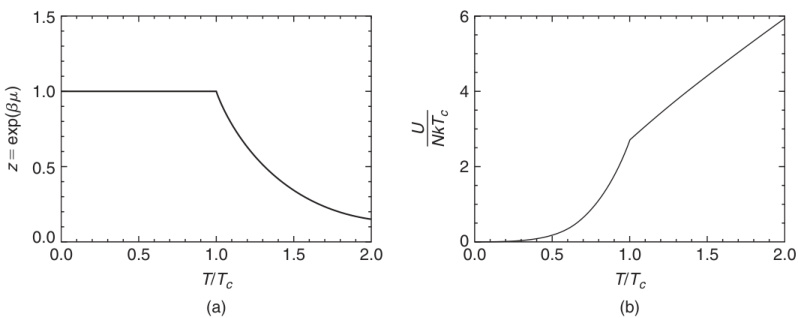
\includegraphics[width=0.71\textwidth]{images/chap7_m802e402f4dec0efe551279e739e9dda7.jpg}
\caption{玻色-爱因斯坦凝聚体在谐振子阱中的 fugacity（a）及缩放温度（\(T/T_c\)）对应的缩放内能（b）。}
\label{fig:7_7.10}
\end{figure}
\begin{figure}[htbp]
\centering
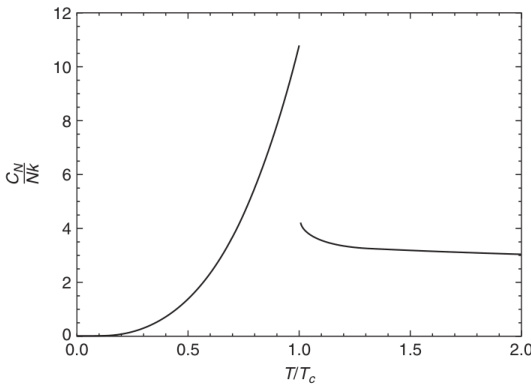
\includegraphics[width=0.47\textwidth]{images/chap7_m5300bbc7a332be8d089e1e5225afc117.jpg}
\caption{玻色-爱因斯坦凝聚体在谐振子阱中的缩放比热随缩放温度（\(T/T_c\)）的变化。}
\label{fig:7_7.11}
\end{figure}
图~\ref{fig:7_7.12} 展示了\(^{87}\)Rb玻色-爱因斯坦凝聚体内能的实验数据。斜率的断裂表明比热具有不连续性。当然，在具有有限粒子数的系统中，所有与相变相关的非解析性都已消除。当 \(N\) 为有限值时，凝聚体分数会平滑地趋近于零，从而使得热容中的不连续性被平滑化。Pathria（1998）推导出了依赖于 \(N\) 的温度标记，这些标记能够根据凝聚体分数和比热来指示玻色-爱因斯坦凝聚的开始；另请参阅Kirsten和Toms（1996）以及Haugerud、Haugest和Ravndal（1997）。
\begin{figure}[htbp]
\centering
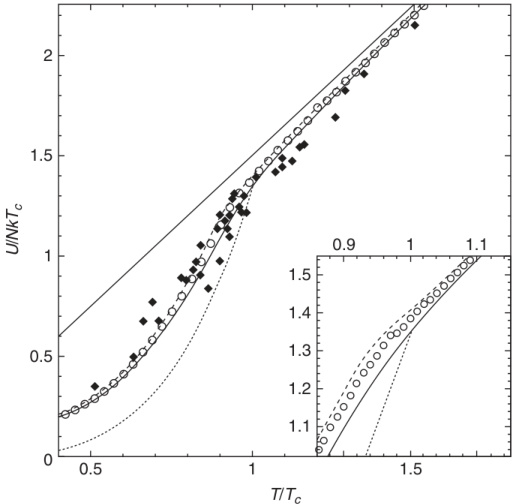
\includegraphics[width=0.46\textwidth]{images/chap7_mfe2d1ae5d5360a08547054f200053320.jpg}
\caption{实验测量值与理论曲线的对比，插图给出临界温度附近放大图。}
\label{fig:7_7.12}
\end{figure}
\section{黑体辐射的热力学}\label{sec:7_3_blackbody}
玻色-爱因斯坦统计学最重要的应用之一，是用于研究黑体辐射的平衡性质。我们考虑一个体积为 \(V\) 的辐射腔，其温度为 \(T\)。从历史上看，该系统一直从两个几乎完全相同但概念上却截然不同的视角加以研究：
\begin{enumerate}
\item 作为由谐振子组成的系统，其能量为量子化的，即 \((n_s+\frac{1}{2})\hbar\omega_s\)，其中 \(n_s=0,1,2,\ldots\)，\(\omega_s\) 是某一谐振子的角频率；
\item 作为由相同且无法区分的量子，即所谓的光子，构成的气体，光子的能量（对应于辐射模式的频率 \(\omega_s\)）为 \(\hbar\omega_s\)。
\end{enumerate}
第一种观点本质上是普朗克在1900年所采用的观点，只不过我们在此还加入了谐振子的零点能；对于辐射的热力学而言，这一能量并不重要，完全可以完全忽略。由于各谐振子彼此可区分（仅凭 \(\omega_{s}\) 的不同值），它们将遵循麦克斯韦-玻尔兹曼统计；然而，单个谐振子的配分函数 \(Q_{1}(V,T)\) 的表达式会与经典表达式有所不同，因为此时谐振子所能达到的能量是离散的，而非连续的；请参阅式（3.8.2） 和 式（3.8.14）。因此，一个频率为 \(\omega_{s}\) 的普朗克谐振子的能量期望值由式（3.8.20） 给出，不包括零点项 \(\frac{1}{2}\hbar\omega_{s}\)：
\begin{equation}\tag{7.2.11}\label{eq:7.2.11}
\langle \varepsilon _ { s } \rangle = \frac { \hbar \omega _ { s } } { e ^{\hbar \omega _ { s} / k T } - 1 } .
\end{equation}
现在，腔体单位体积内，在频率范围 \((\omega, \omega + d\omega)\) 内的正常振动模的数量，由瑞利公式给出
\begin{equation}\tag{7.2.12}\label{eq:7.2.12}
2 \cdot 4 \pi \left( \frac { 1 } { \lambda } \right) ^{2} d \left( \frac { 1 } { \lambda } \right) = \frac { \omega ^{2} d \omega } { \pi ^{2} c ^{3} } ,
\end{equation}
其中已加入因子 2，以考虑横模式的双重性；\(^{11}\) 此处的符号 \(c\) 表示光速。根据\autoref{eq:7.2.11}和\autoref{eq:7.2.12}，与频率范围 \((\omega, \omega + d\omega)\) 相关的能量密度由以下公式给出
\begin{equation}\tag{7.2.13}\label{eq:7.2.13}
u ( \omega ) d \omega = \frac { \hbar } { \pi ^{2} c ^{3} } \, \frac { \omega ^{3} d \omega } { e ^{\hbar \omega / k T} - 1 } ,
\end{equation}
这正是普朗克关于黑体光谱中能量分布的"公式"。通过对 (3) 进行对所有 \(\omega\) 值的积分，我们得到腔体中的总能量密度。
第二种观点源于玻色（1924年）和爱因斯坦（1924年、1925年）。玻色研究了"光子在各个能级间的分布"这一问题；然而，他并没有专注于对各类光子的分配
与其像通常那样将光子分配到各个能级上，他更关注的是能级本身的统计规律！他探讨了诸如"某个能级 \(\varepsilon_{s}=(\hbar\omega_{s})\) 在某一时刻被 \(n_{s}\) 个光子占据的概率"、"\(n_{s}\) 和 \(\varepsilon_{s}\) 的平均值"等问题。实际上，能级的统计规律确实是玻尔兹曼式的；然而，\(n_{s}\) 和 \(\varepsilon_{s}\) 的平均值却会发现
\begin{equation}\tag{7.2.14}\label{eq:7.2.14}
\begin{array}{r} { \langle n _ { s } \rangle = \displaystyle \sum _ { n _ { s } = 0 } ^{\infty} n _ { s } e ^{- n _ { s} \hbar \omega _ { s } / k T } \Bigg / \displaystyle \sum _ { n _ { s } = 0 } ^{\infty} e ^{- n _ { s} \hbar \omega _ { s } / k T } } \\{ = \displaystyle \frac { 1 } { e ^{\hbar \omega _ { s} / k T } - 1 } } \end{array}
\end{equation}
因此，
\begin{equation}\tag{7.2.15}\label{eq:7.2.15}
\langle \varepsilon _ { s } \rangle = \hbar \omega _ { s } \langle n _ { s } \rangle = \frac { \hbar \omega _ { s } } { e ^{\hbar \omega _ { s} / k T } - { \bf 1 } } ,
\end{equation}
与我们先前的结论\autoref{eq:7.2.11}完全一致。为了求得动量介于 \(\hbar\omega/c\) 与 \(\hbar(\omega+d\omega)/c\) 之间的光子态数，玻色借助了这一数与"相空间中相关区域的体积"之间的联系，其结果为
\begin{equation}\tag{7.2.16}\label{eq:7.2.16}
g ( \omega ) d \omega \approx 2 \cdot \frac { V } { h ^{3} } \left\{ 4 \pi \left( \frac { \hbar \omega } { c } \right) ^{2} \left( \frac { \hbar d \omega } { c } \right) \right\} = \frac { V \omega ^{2} d \omega } { \pi ^{2} c ^{3} } ,
\end{equation}
这也与我们先前的结论\autoref{eq:7.2.12}完全一致。因此，他最终得到了普朗克分布公式。需要指出的是，尽管重点在于其他方面，但引导玻色得出最终结果的数学步骤，与振子方法中的步骤在本质上是完全平行的！
另一方面，爱因斯坦更深入地探究了这一问题，并从整体上对光子与能级的统计特性进行了思考。他从玻色的处理方式中推断出：在将光子分配到各个能级的过程中，必须牢记的一个基本事实是：光子彼此无法区分——而这一事实在玻色的处理中早已被隐含地考虑在内。爱因斯坦对所需分布的推导，基本上与第6.1节所给出的推导相同，仅有一个重要区别：由于任意给定体积内的光子总数是不确定的，因此不再存在"固定 N"这一约束条件。由此，拉格朗日乘数 \(\alpha\) 并未参与讨论，也因此，\(\langle n_{\varepsilon} \rangle\) 的最终公式变得更加简洁：
\begin{equation}\tag{7.2.17}\label{eq:7.2.17}
\langle n _ { \varepsilon } \rangle = \frac { 1 } { e ^{\varepsilon / k T} - 1 } ;
\end{equation}
与式（6.1.18a）或（6.2.22）进行比较。上述结果与式（4）完全一致，其中 \(\varepsilon = \hbar\omega_{s}\)。爱因斯坦的后续推导步骤与玻色的推导过程完全相同。
其中
\begin{equation}\tag{7.2.18}\label{eq:7.2.18}
u ^{\prime} ( x ) = \frac { \pi ^{2} \hbar ^{3} c ^{3} } { ( k T ) ^{4} } u ( x )  \mathrm { a n d }  x = \frac { \hbar \omega } { k T } .
\end{equation}
对于长波长情况（\(x \ll 1\)），公式（8）可简化为瑞利（1900年）和詹森（1905年）的经典近似，即\(^{14}\)
\begin{equation}\tag{7.2.19}\label{eq:7.2.19}
u ^{\prime} ( x ) \approx x ^{2} ,
\end{equation}
对于短波长情况（\(x \gg 1\)），其可简化为维恩在1896年提出的著名公式，即
\begin{equation}\tag{7.2.20}\label{eq:7.2.20}
u ^{\prime} ( x ) \approx x ^{3} e ^{- x} .
\end{equation}
与标准的玻色-爱因斯坦结果\autoref{eq:7.1.2}相比，\autoref{eq:7.2.17}表明，我们所面对的情况中，\(z\) 正好等于1。不难看出，这主要是因为本题中粒子的总数量是无限的。因此，它们的平衡数 \(\overline{N}\) 必须由这样一条条件来确定：系统的自由能达到最小值，即 \(\{(\partial A/\partial N)_{N=\overline{N}}\}_{V,T}=0\)。根据定义，这一条件意味着 \(\mu=0\)，从而 \(z=1\)。
若将 \(\langle\varepsilon_{s}\rangle\) 的值采用等分能量的量子理论值（1）而非量子理论值，那么瑞利-詹森公式便能直接推导出来。
为了便于比较，图中还加入了极限形式（10）和（11）。值得注意的是，普朗克曲线与维恩曲线下的面积分别约为 \(\pi^{4}/15 (\simeq 6.49)\) 和 6。然而，瑞利-詹森曲线却饱受高频灾难之苦！
对于腔体内的总能量密度，我们可从方程（8）和（9）中得出
\begin{equation}\tag{7.2.21}\label{eq:7.2.21}
\begin{array}{r} { \frac { U } { V } = \int _ { 0 } ^{\infty} u ( x ) d x = \frac { ( k T ) ^{4} } { \pi ^{2} \hbar ^{3} c ^{3} } \int _ { 0 } ^{\infty} \frac { x ^{3} d x } { e ^{x} - 1 } } \\{ = \frac { \pi ^{2} k ^{4} } { 15 \hbar ^{3} c ^{3} } T ^{4} . } \end{array}
\end{equation}
如果腔体壁上存在一个微小的开口，光子便会"逸出"通过该开口。单位开口面积上的辐射净流速可由下式给出，详见方程（6.4.12），
\begin{equation}\tag{7.2.22}\label{eq:7.2.22}
\frac { 1 } { 4 } \frac { U } { V } c = \frac { \pi ^{2} k ^{4} } { 60 \hbar ^{3} c ^{2} } T ^{4} = \sigma T ^{4} ,
\end{equation}
其中
\begin{equation}\tag{7.2.23}\label{eq:7.2.23}
\sigma = \frac { \pi ^{2} k ^{4} } { 60 \hbar ^{3} c ^{2} } = 5 . 67 0 \times 10 ^{- 8} \mathrm { W m ^{- 2} K ^{- 4} } .
\end{equation}
\autoref{eq:7.2.23}描述了黑体辐射的斯特藩-玻尔兹曼定律，\(\sigma\) 为斯特藩常数。该定律最早由斯特藩于1879年基于实验观测得出；五年后，玻尔兹曼则从热力学角度对其进行了推导。
为进一步研究热力学，我们对光子气体的巨配分函数进行了计算。利用方程（6.2.17），并设 \(z=1\)，我们得到
\begin{equation}\tag{7.2.24}\label{eq:7.2.24}
\ln \mathcal { Q } ( V , T ) \equiv \frac { P V } { k T } = - \sum _ { \varepsilon } \ln ( 1 - e ^{- \varepsilon / k T} ) .
\end{equation}
将求和替换为积分，并借助极端相对论公式
\begin{equation}\tag{7.2.25}\label{eq:7.2.25}
a ( \varepsilon ) d \varepsilon = 2 V \frac { 4 \pi p ^{2} d p } { h ^{3} } = \frac { 8 \pi V } { h ^{3} c ^{3} } \varepsilon ^{2} d \varepsilon ,
\end{equation}
经过部分积分后，我们得到
\begin{equation}\tag{7.2.26}\label{eq:7.2.26}
\ln \mathcal { Q } ( V , T ) \equiv \frac { P V } { k T } = \frac { 8 \pi V } { 3 h ^{3} c ^{3} } \frac { 1 } { k T } \int _ { 0 } ^{\infty} \frac { \varepsilon ^{3} d \varepsilon } { e ^{\varepsilon / k T} - 1 } .
\end{equation}
这里，我们利用了定积分的值为 \(6\zeta(4)=\pi^{4}/15\) 的事实；详情请参见附录D。
通过变量替换，此式变为
\begin{equation}\tag{7.2.27}\label{eq:7.2.27}
\begin{array}{r} { P V = \frac { 8 \pi V } { 3 h ^{3} c ^{3} } ( k T ) ^{4} \int _ { 0 } ^{\infty} \frac { x ^{3} d x } { e ^{x} - 1 } } \\{ = \frac { 8 \pi ^{5} V } { 45 h ^{3} c ^{3} } ( k T ) ^{4} = \frac { 1 } { 3 } U . } \end{array}
\end{equation}
由此我们得到了辐射理论中广为人知的结果——辐射的压力等于其能量密度的三分之一；另请参阅方程（6.4.3）和（6.4.4）。接下来，由于系统的化学势为零，亥姆霍兹自由能等于 \(-PV\)；因此
\begin{equation}\tag{7.2.28}\label{eq:7.2.28}
A = - P V = - { \frac { 1 } { 3 } } U ,
\end{equation}
其中
\begin{equation}\tag{7.2.29}\label{eq:7.2.29}
S \equiv { \frac { U - A } { T } } = { \frac { 4 } { 3 } } { \frac { U } { T } } \propto V T ^{3}
\end{equation}
并且
\begin{equation}\tag{7.2.30}\label{eq:7.2.30}
C _ { V } = T \biggl ( \frac { \partial S } { \partial T } \biggr ) _ { V } = 3 S .
\end{equation}
若辐射经历可逆绝热变化，那么\(T\)与\(V\)的变化规律将遵循如下公式（19），
\begin{equation}\tag{7.2.31}\label{eq:7.2.31}
V T ^{3} = \mathrm { c o n s t . }
\end{equation}
将（21）与\(P \propto T^{4}\)这一事实相结合，我们得到该系统的绝热线方程，即
\begin{equation}\tag{7.2.32}\label{eq:7.2.32}
P V ^{4 / 3} = \mathrm { c o n s t . }
\end{equation}
然而，需要注意的是，光子气体的比值\(C_{P}/C_{V}\)并非4/3；它实际上是无穷大！最后，我们推导出了辐射腔中光子平衡数\(\overline{N}\)的表达式。我们得到
\begin{equation}\tag{7.2.33}\label{eq:7.2.33}
\begin{array}{r} { \overline { { N } } = \frac { V } { \pi ^{2} c ^{3} } \int _ { 0 } ^{\infty} \frac { \omega ^{2} d \omega } { e ^{\hbar \omega / k T} - 1 } } \\{ = V \frac { 2 \zeta ( 3 ) ( k T ) ^{3} } { \pi ^{2} h ^{3} c ^{3} } \propto V T ^{3} . } \end{array}
\end{equation}
尽管该公式颇具启发性，但其不应被简单地视为理所当然，因为在本问题中，由变量\(N\)的波动幅度——而该波动幅度由\((\partial P/\partial V)^{-1}\)这一量决定——是无限大的；参见方程（4.5.7）。
黑体辐射最重要的例子之一便是2.7K的宇宙微波背景辐射，它是大爆炸遗留下来的残余。方程（12）和（23）在我们理解早期宇宙的热力学过程方面发挥着重要作用；请参阅问题7.24以及第九章。
\section{声波领域}\label{ux58f0ux6ce2ux9886ux57df}
与第7.3节所讨论的问题在数学上颇为相似的问题，源于宏观物体——尤其是固体——的振动模式。与黑体辐射的情况类似，固体振动模式的问题同样可以分别从将系统视为谐振子集合，或将其视为一个封闭区域、其中包含声量子气体——即所谓的声子——的角度来加以研究。为了说明这一点，我们以一个由\(N\)个原子构成的经典固体为例，这些原子在空间中的位置由坐标\((x_1, x_2, \ldots, x_{3N})\)来确定。在最低能量状态中，这些坐标的值可表示为\((\overline{x}_1, \overline{x}_2, \ldots, \overline{x}_{3N})\)。将原子偏离其平衡位置的位移\((x_i - \overline{x}_i)\)用变量\(\xi_i (i = 1, 2, \ldots, 3N)\)来表示，则系统在配置\((x_i)\)下的动能可表示为
\begin{equation}\tag{7.4.1}\label{eq:7.4.1}
K = \frac { 1 } { 2 } m \sum _ { i = 1 } ^{3 N} \dot { x } _ { i } ^{2} = \frac { 1 } { 2 } m \sum _ { i = 1 } ^{3 N} \dot { \xi } _ { i } ^{2} ,
\end{equation}
并由势能表示为
\begin{equation}\tag{7.4.2}\label{eq:7.4.2}
\begin{array}{rl} { \Phi \equiv \Phi ( x _ { i } ) = \Phi ( \overline { { x } } _ { i } ) + \sum _ { i } \bigg ( \frac { \partial \Phi } { \partial x _ { i } } \bigg ) _ { ( x _ { i } ) = ( \overline { { x } } _ { i } ) } ( x _ { i } - \overline { { x } } _ { i } ) } & { } \\{ + \sum _ { i , j } \frac { 1 } { 2 } \bigg ( \frac { \partial ^{2} \Phi } { \partial x _ { i } \partial x _ { j } } \bigg ) _ { ( x _ { i } ) = ( \overline { { x } } _ { i } ) } ( x _ { i } - \overline { { x } } _ { i } ) ( x _ { j } - \overline { { x } } _ { j } ) + \cdots . } & { } \end{array}
\end{equation}
本展开式中的主项表示在所有原子均处于其平均位置\(\bar{x}_{i}\)且静止时，固体所具有的（最小）能量；该能量可记作\(\Phi_{0}\)。接下来的项因函数\(\Phi(x_{i})\)在\((x_{i})=(\bar{x}_{i})\)处取得极小值，因此其一阶导数在该点为零，故各项均为零。展开式的二阶项代表了原子围绕其平均位置振动的谐振分量。若我们假设这些振动的总体振幅并不大，则可仅保留展开式的谐振项，而忽略后续的各项；此时我们便处于所谓的谐振近似之中。由此，我们可以写出
\begin{equation}\tag{7.4.3}\label{eq:7.4.3}
H = \Phi _ { 0 } + \left\{ \sum _ { i } \frac { 1 } { 2 } m \dot { \xi } _ { i } ^{2} + \sum _ { i , j } \alpha _ { i j } \dot { \xi } _ { i } \dot { \xi } _ { j } \right\} ,
\end{equation}
其中
\begin{equation}\tag{7.4.4}\label{eq:7.4.4}
\alpha _ { i j } = \frac { 1 } { 2 } \left( \frac { \partial ^{2} \Phi } { \partial x _ { i } \partial x _ { j } } \right) _ { ( x _ { i } ) = ( \overline { { x } } _ { i } ) } .
\end{equation}
现在我们引入一种线性变换，将坐标\(\xi_{i}\)转换为所谓的正则坐标\(q_{i}\)，并选择变换矩阵，使得哈密顿量的新表达式中不包含任何交叉项，即，
\begin{equation}\tag{7.4.5}\label{eq:7.4.5}
H = \Phi _ { 0 } + \sum _ { i } \frac { 1 } { 2 } m \Big ( \dot { q } _ { i } ^{2} + \omega _ { i } ^{2} q _ { i } ^{2} \Big ) ,
\end{equation}
其中\(\omega_{i}(i=1,2,\ldots,3N)\)是系统的正则模态的特征频率，其本质上由\(\alpha_{ij}\)这一参数决定，或者进一步由势能函数\(\Phi(x_{i})\)的性质所决定。\autoref{eq:7.4.5}表明，固体的能量在\((最小)\)值\(\Phi_{0}\)之外的部分，可以被视为由一组\(3N\)个一维、非相互作用、谐振子所构成，而这些谐振子的特征频率\(\omega_{i}\)则由系统内的原子间相互作用决定。
从经典力学的角度来看，\(3N\)个正则模态对应于晶格的一种畸变波，亦即声波。而在量子力学中，这些模态会激发出称为声子的量子，其产生方式与电磁场的振动模态激发光子的方式大致相同。然而，两者之间存在一个重要的区别：对于电磁场而言，其正则模态的数量是无限的；而对于固体而言，正则模态的数量（或声子能级的数量）则由晶格位点的数量所限定。这使得声场的热力学行为与辐射场的热力学行为呈现出一定的差异；不过，在低温条件下，当固体的高频模态不太可能被激发时，这些差异便变得微不足道，我们最终会发现，这两组结果之间存在着惊人的相似性。
如今，固体的热力学研究可以沿第3.8节的思路展开。首先，我们注意到哈密顿量(5)的特征值为
\begin{equation}\tag{7.4.6}\label{eq:7.4.6}
E \{ n _ { i } \} = \Phi _ { 0 } + \sum _ { i } \Big ( n _ { i } + \frac { 1 } { 2 } \Big ) \hbar \omega _ { i } ,
\end{equation}
其中，各振子的"激发态"数值 \(n_{i}\) 表示了系统中各振子的"激发态"（或 equivalently，表示系统中各声子能级的占据数）。系统的内能则可表示为
\begin{equation}\tag{7.4.7}\label{eq:7.4.7}
U ( T ) = \left\{ \Phi _ { 0 } + \sum _ { i } \frac { 1 } { 2 } \hbar \omega _ { i } \right\} + \sum _ { i } \frac { \hbar \omega _ { i } } { e ^{\hbar \omega _ { i} / k T } - 1 } .
\end{equation}
当然，声子本身的数量是无限的。因此，声子气体的化学势也为零。
括号内的表达式给出了在绝对零度下固体的能量。项 \(\Phi_{0}\) 为负值，且其大小远大于振子的总零点能——\(\sum_{i\frac{1}{2}}\hbar\omega_{i}\)——二者共同决定了晶格的结合能。\autoref{eq:7.4.7} 中的最后一项代表了能量中随温度变化的部分，\(^{17}\) 这一项决定了固体的比热：
\begin{equation}\tag{7.4.8}\label{eq:7.4.8}
C _ { V } ( T ) \equiv \left( \frac { \partial U } { \partial T } \right) _ { V } = k \sum _ { i } \frac { ( \hbar \omega _ { i } / k T ) ^{2} e ^{\hbar \omega _ { i} / k T } } { ( e ^{\hbar \omega _ { i} / k T } - 1 ) ^{2} } .
\end{equation}
要进一步推进研究，我们需要了解固体的频率谱。要从基本原理出发获得这一频谱并非易事。因此，我们通常通过实验来获取该频谱，或者基于对频谱的某些合理假设来进行推导。爱因斯坦率先将量子概念应用于固体理论（1907年），为了简化起见，他假设所有频率 \(\omega_{i}\) 都相等。将这一（普遍）值记作 \(\omega_{E}\)，固体的比热可表示为
\begin{equation}\tag{7.4.9}\label{eq:7.4.9}
C _ { V } ( T ) = 3 N k E ( x ) ,
\end{equation}
其中，\(E(x)\) 即所谓的爱因斯坦函数：
\begin{equation}\tag{7.4.10}\label{eq:7.4.10}
E ( x ) = \frac { x ^{2} e ^{x} } { ( e ^{x} - 1 ) ^{2} } ,
\end{equation}
其中
\begin{equation}\tag{7.4.11}\label{eq:7.4.11}
x = \hbar \omega _ { E } / k T = \Theta _ { E } / T .
\end{equation}
图~7.14 中的虚线曲线展示了比热随温度的变化情况，其依据为爱因斯坦公式\autoref{eq:7.4.9}。在温度足够高的情况下，即 \(T \gg \Theta_E\)，因而 \(x \ll 1\) 时，爱因斯坦的结果趋于经典结果，即 \(3Nk\)。而在温度足够低的情况下，即 \(T \ll \Theta_E\)，因而 \(x \gg 1\) 时，比热会以指数级的速度下降，并随着 \(T \to 0\) 而趋近于零。然而，根据理论计算所得的下降速率，与实际观测到的下降速率相比显得过快。尽管如此，爱因斯坦的方法至少为理解固体比热偏离经典杜朗-佩蒂定律提供了理论基础——按照该定律，\(C_V = 3R \simeq 5.96\) 卡路里每摩尔每摄氏度。
另一方面，德拜（1912年）则允许存在连续的频率谱，并将其上限设定为 \(\omega_{D}\)，使得振动正常模式的总数为 \(3N\)。
其中，\(g(\omega)d\omega\) 表示频率位于区间 \((\omega, \omega + d\omega)\) 内的正常振动模式的数量。对于 \(g(\omega)\)，德拜采用了瑞利公式（7.3.2），并对其进行了修正，以适应所研究的问题。设 \(c_L\) 为纵波传播速度，\(c_T\) 为横波传播速度（并注意到，对于任意频率 \(\omega\)，横波模式均为双重简并），则方程（12）变为
\begin{equation}\tag{7.4.12}\label{eq:7.4.12}
\int _ { 0 } ^{\omega D} V \left( \frac { \omega ^{2} d \omega } { 2 \pi ^{2} c _ { L } ^{3} } + \frac { \omega ^{2} d \omega } { \pi ^{2} c _ { T } ^{3} } \right) = 3 N ,
\end{equation}
由此可得截止频率
\begin{equation}\tag{7.4.13}\label{eq:7.4.13}
\omega _ { D } ^{3} = 18 \pi ^{2} \frac { N } { V } \left( \frac { 1 } { c _ { L } ^{3} } + \frac { 2 } { c _ { T } ^{3} } \right) ^{- 1} .
\end{equation}
因此，德拜谱可以写成
\begin{equation}\tag{7.4.14}\label{eq:7.4.14}
g ( \omega ) = \left\{ \begin{array}{ll} { \displaystyle \frac { 9 N } { \omega _ { D } ^{3} } \omega ^{2} } & { \mathrm { f o r ~ } \omega \leq \omega _ { D } , } \\{ 0 } & { \mathrm { f o r ~ } \omega > \omega _ { D } . } \end{array} \right.
\end{equation}
在进一步依据德拜谱计算固体比热之前，我们似乎有必要先作两点说明。首先，德拜谱只是对固体中实际现象的一种理想化描述；例如，它可以与图~7.15 所示的典型谱进行比较。尽管对于低频模式（即所谓的声学模式），德拜近似是合理的，但在高频模式（即所谓的光学模式）的情况下，却出现了严重的偏差。在\ldots\ldots{}
无论如何，对于诸如比热等"平均"量而言，谱的精细细节并不十分重要。其次，固体的纵波模式和横波模式应各自拥有各自的截止频率，例如 \(\omega_{D,L}\) 和 \(\omega_{D,T}\)，而非采用统一的截止频率 \(\omega_{D}\)，原因很简单：在晶格的 \(3N\) 个正常模式中，恰好有 \(N\) 个是纵波模式，而 \(2N\) 个是横波模式。因此，我们应当采用的公式并非（13），
\begin{equation}\tag{7.4.15}\label{eq:7.4.15}
\int _ { 0 } ^{\omega _ { D , L} } V \frac { \omega ^{2} d \omega } { 2 \pi ^{2} c _ { L } ^{3} } = N  \mathrm { a n d }  \int _ { 0 } ^{\omega _ { D , T} } V \frac { \omega ^{2} d \omega } { \pi ^{2} c _ { T } ^{3} } = 2 N .
\end{equation}
我们注意到，这两个截止频率对应于共同的波长 \(\lambda_{\mathrm{min}} = \left( \frac{4\pi V}{3N} \right)^{1/3}\)，这一波长与固体中的平均原子间距离相当。这是相当合理的，因为当波长短于 \(\lambda_{\mathrm{min}}\) 时，若再谈论原子位移的波，就显得有些无意义了。
在德拜近似下，\autoref{eq:7.4.8}给出
\begin{equation}\tag{7.4.16}\label{eq:7.4.16}
C _ { V } ( T ) = 3 N k D ( x _ { 0 } ) ,
\end{equation}
其中 \(D(x_0)\) 是所谓的德拜函数：
\begin{equation}\tag{7.4.17}\label{eq:7.4.17}
D ( x _ { 0 } ) = \frac { 3 } { x _ { 0 } ^{3} } \int _ { 0 } ^{x _ { 0} } \frac { x ^{4} e ^{x} d x } { ( e ^{x} - 1 ) ^{2} } ,
\end{equation}
其中
\begin{equation}\tag{7.4.18}\label{eq:7.4.18}
x _ { 0 } = \frac { \hbar \omega _ { D } } { k T } = \frac { \Theta _ { D } } { T } ,
\end{equation}
\(\Theta_{D}\) 即为固体的所谓德拜温度。通过分部积分，德拜函数的表达式变为
\begin{equation}\tag{7.4.19}\label{eq:7.4.19}
D ( x _ { 0 } ) = - \frac { 3 x _ { 0 } } { e ^{x _ { 0} } - 1 } + \frac { 12 } { x _ { 0 } ^{3} } \int _ { 0 } ^{x _ { 0} } \frac { x ^{3} d x } { e ^{x} - 1 } .
\end{equation}
对于 \(T \gg \Theta_{D}\)，即 \(x_{0} \ll 1\) 的情形，函数 \(D(x_{0})\) 可以表示为 \(x_{0}\) 的幂级数：
\begin{equation}\tag{7.4.20}\label{eq:7.4.20}
D ( x _ { 0 } ) = 1 - { \frac { x _ { 0 } ^{2} } { 20 } } + \cdots .
\end{equation}
因此，当 \(T \to \infty\) 时，\(C_V \to 3Nk\)；此外，根据这一理论，只要 \(T > 3\Theta_D\)，经典结果就应能适用于误差不超过 \(\frac{1}{2}\)\% 的范围。而对于 \(T \ll \Theta_D\)，即 \(x_0 \gg 1\) 的情形，函数 \(D(x_0)\) 可以写成：
\begin{equation}\tag{7.4.21}\label{eq:7.4.21}
\begin{array}{r} { D ( x _ { 0 } ) = \frac { 12 } { x _ { 0 } ^{3} } \int _ { 0 } ^{\infty} \frac { x ^{3} d x } { e ^{x} - 1 } + O ( e ^{- x _ { 0} } ) , } \\{ \approx \frac { 4 \pi ^{4} } { 5 x _ { 0 } ^{3} } = \frac { 4 \pi ^{4} } { 5 } \left( \frac { T } { \Theta _ { D } } \right) ^{3} . } \end{array}
\end{equation}
因此，在低温下，固体的比热遵循德拜 \(T^{3}\) 定律：
\begin{equation}\tag{7.4.22}\label{eq:7.4.22}
C _ { V } = \frac { 12 \pi ^{4} } { 5 } N k \biggl ( \frac { T } { \Theta _ { D } } \biggr ) ^{3} = 46 4 . 4 \biggl ( \frac { T } { \Theta _ { D } } \biggr ) ^{3} \mathrm { c a l \ m o l e } ^{- 1} \mathrm { K } ^{- 1} .
\end{equation}
从\autoref{eq:7.4.22}中可以清楚地看出，对固体进行低温比热测量，不仅能够验证 \(T^{3}\) 定律的正确性，还能获得德拜温度 \(\Theta_{D}\) 的经验值。19 德拜温度 \(\Theta_{D}\) 的数值，也可以通过已知参数 \(N/V\)、\(c_{L}\) 和 \(c_{T}\) 来计算出截止频率 \(\omega_{D}\)；具体见式（14）和式（19）。这些估算值之间的高度吻合，进一步证明了德拜理论的合理性。一旦得知 \(\Theta_{D}\) 的值，便可通过利用表格中列出的函数 \(D(x_{0})\) 的数值，从理论上覆盖整个温度范围。20 一个典型的例子已在图~7.14 中展示过。我们发现，不仅在低温下 \(T^{3}\) 定律依然成立，而且在整个观测范围内，理论与实验之间的拟合度都相当理想。
19 可以证明，根据这一理论，在 \(T < \Theta_{D}/10\) 的范围内，偏离 \(T^{3}\) 定律的幅度不应超过 2\%。然而，对于金属而言，我们无法期待真正达到 \(T^{3}\) 区域，因为早在该区域之前，电子气体的比热就可能成为主导贡献因素（参见第 8.3 节）；除非将这两种贡献区分开来，否则我们很可能会从这些观测中得到一个略显被抑制的 \(\Theta_{D}\) 值。
20 例如，请参阅 Fowler 和 Guggenheim（1960，第 144 页）。
作为低温区域一致性的一个又一例证，我们在此附上另一幅图——图~7.16，该图基于在低于 5K 温度下使用 KCl 晶体所获得的数据；请参阅 Keesom 和 Pearlman（1953）。图中，\(C_{V}/T\) 的观测值被绘制于 \(T^{2}\) 坐标系中。显然，这些数据很好地落在一条直线上，而通过该直线的斜率，便可确定 \(\Theta_{D}\) 的值。因此，对于 KCl，我们得到 \(\Theta_{D} = 233 \pm 3\)K，这一结果与各处相关弹性常数估计值所得到的 230 至 246 K 值基本一致。
在表 7.1 中，我们列出了若干晶体的 \(\Theta_{D}\) 值，这些值分别来自比热测量以及弹性常数的测定结果。
一般来说，如果某一特定系统的比热测量结果符合 \(T^3\) 规律，那么可以推断该系统中的热激发完全由声子所负责。我们同样预期，在液体中也会发生类似的现象，但存在两个重要的差异。首先，由于液体无法承受剪切应力，因此无法维持横向振动模式；因此，由 \(N\) 个原子组成的液体，仅具有 \(N\) 个纵向振动模式。其次，液体的正常模式并不一定严格呈谐振状态；因此，除了声子之外，我们还可能遇到其他类型的激发，例如涡流流动或湍流（甚至还有某种改良型的激发，如液态氦 \(^{4}\) 中的罗通子）。
其中，
\begin{equation}\tag{7.4.23}\label{eq:7.4.23}
\omega _ { D } = \left( \frac { 6 \pi ^{2} N } { V } \right) ^{1 / 3} c ,
\end{equation}
\(c\) 为液体中的声速。液体单位质量的比热则可表示为
\begin{equation}\tag{7.4.24}\label{eq:7.4.24}
c _ { V } = \frac { 2 \pi ^{2} k ^{4} } { 15 \rho \hbar ^{3} c ^{3} } T ^{3} ,
\end{equation}
其中，\(\rho\) 为质量密度。将 \(\rho = 0.1455\,\mathrm{g/cm}^3\) 和 \(c = 238\,\mathrm{m/s}\) 代入，上述结果变为
\begin{equation}\tag{7.4.25}\label{eq:7.4.25}
c _ { V } = 0 . 02 09 T ^{3} \mathrm { j o u l e g } ^{- 1} \mathrm { K } ^{- 1} .
\end{equation}
Wiebes 等人（1957）在 \(0 < T < 0.6\)K 时的实验测量结果，均符合以下表达式
\begin{equation}\tag{7.4.26}\label{eq:7.4.26}
c _ { V } = ( 0 . 02 04 \pm 0 . 00 04 ) T ^{3} \mathrm { j o u l e g } ^{- 1} \mathrm { K } ^{- 1} .
\end{equation}
理论结果与实验观测之间的吻合度显然相当高。
\section{声场的惯性密度}\label{ux58f0ux573aux7684ux60efux6027ux5bc6ux5ea6}
为了进一步理解液态氦\(^{4}\)的低温行为，我们对处于热平衡状态的声子气体所对应的"惯性质量"进行了测定。为此，我们以"处于质量运动中的声子气体"为研究对象；通过确定该气体的动量\(P\)与质量运动速度\(\nu\)之间的关系，我们便能轻松地计算出所要研究的这一性质。由于系统中声子的总数是不确定的，因此问题并不受固定\(N\)的约束；相应地，未定乘数\(\alpha\)可以被取为零。然而，我们如今又为系统新增了一项约束条件——即总动量\(P\)的固定，除此之外，
总能量\(E\)的固定约束。在这些约束条件下，声子能级\(\varepsilon(\boldsymbol{p})\)的平均占据数将为
\begin{equation}\tag{7.5.1}\label{eq:7.5.1}
\langle n ( p ) \rangle = \frac { 1 } { \exp ( \beta \varepsilon + \gamma \cdot p ) - 1 } .
\end{equation}
如同往常一样，参数\(\beta\)等于\(1/kT\)。为了确定\(\gamma\)，我们似乎自然地选择评估气体的漂移速度。若以质量运动方向为z轴，则漂移速度的大小\(\nu\)可由"单个声子速度中\(u_z\)分量的平均值"给出：
\begin{equation}\tag{7.5.2}\label{eq:7.5.2}
\nu = \langle u \cos \theta \rangle .
\end{equation}
现在，对于声子而言，
\begin{equation}\tag{7.5.3}\label{eq:7.5.3}
\varepsilon = p c  \mathrm { a n d }  u \equiv \frac { d \varepsilon } { d p } = c ,
\end{equation}
其中\(c\)为介质中的声速。此外，出于对称性的考虑，我们预期未定向量\(\boldsymbol{\gamma}\)要么与质量运动方向平行，要么与之反平行；因此，我们可以写成
\begin{equation}\tag{7.5.4}\label{eq:7.5.4}
\gamma \cdot p = \gamma _ { z } p _ { z } = \gamma _ { z } p \cos \theta .
\end{equation}
鉴于\autoref{eq:7.5.1}、\autoref{eq:7.5.3}和\autoref{eq:7.5.4}，\autoref{eq:7.5.2}变为
\begin{equation}\tag{7.5.5}\label{eq:7.5.5}
\nu = \frac { \int _ { 0 } ^{\infty} \int _ { 0 } ^{\pi} [ \exp \{ \beta p c ( 1 + ( \gamma _ { z } / \beta c ) \cos \theta ) \} - 1 ] ^{- 1} ( c \cos \theta ) ( p ^{2} d p 2 \pi \sin \theta d \theta ) } { \int _ { 0 } ^{\infty} \int _ { 0 } ^{\pi} [ \exp \{ \beta p c ( 1 + ( \gamma _ { z } / \beta c ) \cos \theta ) \} - 1 ] ^{- 1} ( p ^{2} d p 2 \pi \sin \theta d \theta ) } .
\end{equation}
进行替换
\begin{equation}\tag{7.5.6}\label{eq:7.5.6}
\cos \theta = \eta ,  p ( { \bf 1 } + ( \gamma _ { z } / \beta c ) \eta ) = p ^{\prime}
\end{equation}
并消去对\(p'\)的积分，我们得到
\begin{equation}\tag{7.5.7}\label{eq:7.5.7}
\nu = c \frac { \int _ { - 1 } ^{1} ( 1 + ( \gamma _ { z } / \beta c ) \eta ) ^{- 3} \eta d \eta } { \int _ { - 1 } ^{1} ( 1 + ( \gamma _ { z } / \beta c ) \eta ) ^{- 3} d \eta } = - \gamma _ { z } / \beta .
\end{equation}
由此可知，
\begin{equation}\tag{7.5.8}\label{eq:7.5.8}
\gamma = - \beta v .
\end{equation}
据此，平均占据数的表达式变为
\begin{equation}\tag{7.5.9}\label{eq:7.5.9}
\langle n ( p ) \rangle = \frac { 1 } { \exp \{ \beta ( \varepsilon - v \cdot p ) \} - 1 } .
\end{equation}
将\autoref{eq:7.5.9}与气体静止参考系中的对应结果进行比较，即
\begin{equation}\tag{7.5.10}\label{eq:7.5.10}
\langle n _ { 0 } ( p _ { 0 } ) \rangle = \frac { 1 } { \exp ( \beta \varepsilon _ { 0 } ) - 1 } ,
\end{equation}
可以看出，通过施加质量运动对系统造成的改变，不过是两种参考系之间伽利略变换的直观体现。
或者，\autoref{eq:7.5.9}也可以写成
\begin{equation}\tag{7.5.11}\label{eq:7.5.11}
\langle n ( p ) \rangle = \frac { 1 } { \exp ( \beta p ^{\prime} c ) - 1 } = \frac { 1 } { \exp \{ \beta p c ( 1 - ( \nu / c ) \cos \theta ) \} - 1 } .
\end{equation}
因此，\autoref{eq:7.5.9}对漂移速度\(\nu\)作出了严格的限制——即，\(\nu\)不得超过声子的速度\(c\)，否则部分占据数将变为负值！事实上，正如我们后续的分析所表明的那样，当\(\nu\)接近\(c\)时，本节所建立的理论框架将失效。因此，声子气体的流动速度\(c\)可被视为临界速度：
\begin{equation}\tag{7.5.12}\label{eq:7.5.12}
( \nu _ { c } ) _ { \mathrm { p h } } = c .
\end{equation}
这一结果与液氦II超流性问题之间的关联将在下一部分中得到阐明。
接下来，我们计算声子气体的总动量\(P\)：
\begin{equation}\tag{7.5.13}\label{eq:7.5.13}
P = \sum _ { p } \langle n ( p ) \rangle p .
\end{equation}
事实上，向量\(P\)将与向量\(v\)平行，而后者本身已沿\(z\)轴方向运动。因此，我们只需计算动量的\(z\)分量：
\begin{equation}\tag{7.5.14}\label{eq:7.5.14}
\begin{aligned} P & = P _ { z } = \sum _ { p } \langle n ( p ) \rangle p _ { z } \\& = \int _ { 0 } ^{\infty} \int _ { 0 } ^{\pi} \frac { p \cos \theta } { \exp \{ \beta p c ( 1 - ( v / c ) \cos \theta ) \} } - 1 \left( \frac { V p ^{2} d p 2 \pi \sin \theta d \theta } { h ^{3} } \right) \\& = \frac { 2 \pi V } { h ^{3} } \int _ { 0 } ^{\infty} \frac { p ^{\prime 3} d p ^{\prime} } { \exp ( \beta p ^{\prime} c ) - 1 } \int _ { 0 } ^{\pi} \{ 1 - ( v / c ) \cos \theta \} ^{- 4} \cos \theta \sin \theta d \theta \\& = V \frac { 16 \pi ^{5} } { 45 h ^{3} c ^{3} \beta ^{4} } \cdot \frac { v / c ^{2} } { ( 1 - v ^{2} / c ^{2} ) ^{3} } . \end{aligned}
\end{equation}
气体的总能量\(E\)由以下公式给出：
\begin{equation}\tag{7.5.15}\label{eq:7.5.15}
\begin{array}{rl} & { E = \sum _ { p } \langle n ( p ) \rangle p c } \\& {  = \frac { 2 \pi \, V c } { h ^{3} } \int _ { 0 } ^{\infty} \frac { p ^{\prime 3} \, d p ^{\prime} } { \exp ( \beta p ^{\prime} c ) - 1 } \int _ { 0 } ^{\pi} \{ 1 - ( v / c ) \cos \theta \} ^{- 4} \sin \theta d \theta } \\& {  = V \frac { 4 \pi ^{5} } { 15 h ^{3} c ^{3} \beta ^{4} } \frac { 1 + \frac { 1 } { 3 } v ^{2} / c ^{2} } { ( 1 - v ^{2} / c ^{2} ) ^{3} } . } \end{array}
\end{equation}
自然地，我们将\(P/\nu\)的比值视为声子气体的"惯性质量"。相应地，其质量密度\(\rho\)则由以下公式给出：
\begin{equation}\tag{7.5.16}\label{eq:7.5.16}
\rho = \frac { P } { v V } = \frac { 16 \pi ^{5} k ^{4} T ^{4} } { 45 h ^{3} c ^{5} } \frac { 1 } { ( 1 - v ^{2} / c ^{2} ) ^{3} } .
\end{equation}
对于\((v/c) \ll 1\)的情况——通常情况下确实如此——声子气体的质量密度可表示为：
\begin{equation}\tag{7.5.17}\label{eq:7.5.17}
( \rho _ { 0 } ) _ { \mathrm { p h } } = \frac { 16 \pi ^{5} k ^{4} } { 45 h ^{3} c ^{5} } T ^{4} = \frac { 4 } { 3 c ^{2} } ( E _ { 0 } / V ) .
\end{equation}
将液氦\(^{4}\)在低温下的声子质量密度代入公式，该质量密度相对于液体的实际密度而言，可表示为：
\begin{equation}\tag{7.5.18}\label{eq:7.5.18}
( \rho _ { 0 } ) \mathrm { p h } / \rho _ { \mathrm { H e } } = 1 . 22 \times 10 ^{- 4} T ^{4} ;
\end{equation}
例如，在\(T=0.3\mathrm{K}\)时，这一比值约为\(9.9\times10^{-7}\)。而在如\(0.3\mathrm{K}\)这样的温度下，声子是液氦\(^{4}\)中唯一需要考虑的激发态；因此，计算所得的结果应与"液态正常流体的密度\(\rho_{n}\)与液态总密度\(\rho\)之比"相对应。要直接精确地确定如此微小的比值几乎是不可能的；然而，借助其他实验上可行的液体性质进行间接估算，却为上述结果提供了有力的证实——详见图~7.17。
第7.6节 液氦II中的基本激发态
朗道（1941年、1947年）提出了一套简单的理论框架，能够较好地解释液氦II在低温下、且未过于靠近\(\lambda\)点时的行为。根据这一框架，液态被视作一个弱激发的量子力学系统，在该系统中，从基态（\(T = 0\mathrm{K}\)）出发的偏离，可通过"悬浮于静止背景之上的基本激发态气体"来加以描述。激发态气体对应于"正常流体"，而静止背景则代表"超流体"。
因此，在\(T=T_{\lambda}\)时，\(\rho_{n}=\rho_{\mathrm{He}}\)，而\(\rho_{s}=0\)。当\(T>T_{\lambda}\)时，液体在各方面都表现为普通流体，即我们通常所熟知的液态氦I。
基于纯粹的经验性考量，朗道还提出了液态氦II中基本激发态的能量-动量关系\(\varepsilon(p)\)。在低动量下，\(\varepsilon\)与\(p\)之间的关系呈线性（这正是声子的典型特征），而在高动量下，则呈现出非单调的特性。这些激发态被假定为玻色子，并且在低温下（此时激发态的数量并不算多）彼此之间互不相互作用；随后，通过采用一种简单直接的统计力学方法，便可计算出液体的宏观性质。研究发现，朗道的理论能够相当成功地解释液态氦II在约0至2K温度范围内的观测性质；然而，仍需进一步验证，液体中的实际激发态是否真的符合所提出的能量谱。
在科恩和费曼（1957年）的建议指导下，多位实验工作者着手通过散射长波长中子（\(\lambda \gtrsim 4\text{\AA}\)）来研究液态氦II中的激发态能谱。在低于2K的温度下，最重要的散射过程是中子在液体中产生单个激发态的过程。通过测量在某一角度\(\phi\)下散射的中子的修正波长\(\lambda_{f}\)，便可以确定在散射过程中产生的激发态的能量\(\varepsilon\)和动量\(p\)。
可根据相关守恒定律加以确定：
\begin{equation}\tag{7.5.19}\label{eq:7.5.19}
\varepsilon = h ^{2} ( \lambda _ { i } ^{- 2} - \lambda _ { f } ^{- 2} ) / 2 m ,
\end{equation}
\begin{equation}\tag{7.5.20}\label{eq:7.5.20}
p ^{2} = h ^{2} ( \lambda _ { i } ^{- 2} + \lambda _ { f } ^{- 2} - 2 \lambda _ { i } ^{- 1} \lambda _ { f } ^{- 1} \cos \phi ) ,
\end{equation}
其中\(\lambda_{i}\)为中子的初始波长，\(m\)为中子质量。通过改变\(\phi\)，或\(\lambda_{i}\)，便可绘制出激发态的完整能谱。
首次沿着这一方向展开的全面研究由亚内尔等人（1959年）完成；他们的研究成果如图~7.18所示，与朗道所提出的经验能谱有着惊人的相似之处。在1.1K温度下获得的能谱中，较为重要的特征如下：
（i）如果我们对位于 \(p/\hbar = 0.55\text{\AA}^{-1}\) 周围的点拟合线性、类声子谱（\(\varepsilon = pc\)），则可得 \(c\) 的值为 \((239 \pm 5)\,\mathrm{m/s}\)，这一结果与液体中声速的实测值——约 \(238\,\mathrm{m/s}\)——高度吻合。
（ii）该谱在 \(\varepsilon/k = (13.92 \pm 0.10)\text{\AA}^{-1}\) 处通过一个最大值。
（iii）随后，在 \(p/\hbar = (1.92 \pm 0.01)\text{\AA}^{-1}\) 处出现一个最小值，其邻近区域可由朗道的罗通能谱来描述：
\begin{equation}\tag{7.5.21}\label{eq:7.5.21}
\varepsilon ( p ) = \Delta + \frac { ( p - p _ { 0 } ) ^{2} } { 2 \mu } ,
\end{equation}
与
\begin{equation}\tag{7.5.22}\label{eq:7.5.22}
\begin{array}{r} { \Delta / k = ( 8 . 65 \pm 0 . 04 ) \mathrm { K } , } \\{ p _ { 0 } / \hbar = ( 1 . 92 \pm 0 . 01 ) \text { \AA } ^{- 1} , } \end{array}
\end{equation}
以及
\begin{equation}\tag{7.5.23}\label{eq:7.5.23}
\mu = ( 0 . 16 \pm 0 . 01 ) m _ { \mathrm { H e } } .
\end{equation}
（iv）在 \(p/\hbar \simeq 2.18\text{\AA}^{-1}\) 以上，谱线呈线性上升，且斜率仍为 \(c\)。我们还分别在1.6K和1.8K的温度下获得了数据。发现该谱的总体形状与1.1K时基本一致；仅 \(\Delta\) 的数值略低一些。
在后续研究中，Henshaw 和 Woods（1961）将观测范围扩展到了谱线两端；他们的研究成果见图~7.19。在谱线的较低端，他们将测量范围一直延伸至 \(p/\hbar = 0.26\text{\AA}^{-1}\)，并发现实验所得的
\^{}\{21\}"罗通"这一术语是朗道提出的，他最初认为这些激发态或许能在某种程度上代表液体中一种旋转性质的局域扰动。然而，后续的理论研究，尤其是费曼（1953、1954）以及布鲁克纳和泽瓦达（1957）的研究，并未支持这一观点。尽管如此，"罗通"这一术语仍被沿用至今。
这些点确实位于一条直线上（斜率为237 m/s）。在谱线的较高端，他们将测量范围进一步拓展至 \(p/\hbar=2.68\text{\AA}^{-1}\)，并发现：在经过1.91\(\text{\AA}^{-1}\) 处的最小值后，曲线以不断增大的斜率向上延伸，直至大约2.4\(\text{\AA}^{-1}\)，此时二阶导数 \(\partial^2\varepsilon/\partial p^2\) 发生符号反转；曲线随后的趋势表明，谱线中可能存在第二个最大值！22
要对液氦II的热力学性质进行评估，我们首先注意到，在温度足够低的情况下，我们仅存在一些低能激发态，即声子。液态的热力学行为随后由第7.4节和第7.5节中推导出的公式所支配。当温度高于约0.5K时，第二类激发态——即罗通子（其动量接近\(p_0\)）——也会出现。在0.5K与约1K之间，液态的行为由声子与罗通子共同决定。然而，当温度高于1K时，声子对液态各项热力学性质的贡献已变得相当微弱；此时，只有罗通子需要被纳入考量。
接下来，我们将研究罗通子对液态各项热力学性质的温度依赖性。鉴于能谱具有连续性，人们自然会预期，如同声子一样，罗通子也遵循玻色-爱因斯坦统计。此外，系统中罗通子的总数量\(N\)是相当不确定的；因此，它们的化学势\(\mu\)恒为零。于是，我们得到罗通子的平均占据数为：
\begin{equation}\tag{7.5.24}\label{eq:7.5.24}
\langle n ( p ) \rangle = \frac { 1 } { \exp \{ \beta \varepsilon ( p ) \} - 1 } ,
\end{equation}
其中，\(\varepsilon(p)\)由\autoref{eq:7.5.4}和\autoref{eq:7.5.5}给出。在所有我们所关心的温度下（即\(T \leq 2\)K），项\(\exp\{\beta\varepsilon(p)\}\)的最小值——即\(\exp(\Delta/kT)\)——远远大于1。因此，我们可以写成：
\begin{equation}\tag{7.5.25}\label{eq:7.5.25}
\langle n ( p ) \rangle \simeq \exp \{ - \beta \varepsilon ( p ) \} .
\end{equation}
因此，罗通子系统的\(q\)势可表示为：
\begin{equation}\tag{7.5.26}\label{eq:7.5.26}
q ( V , T ) \equiv \frac { P V } { k T } = - \sum _ { p } \ln [ 1 - \exp \{ - \beta \varepsilon ( p ) \} ] \simeq \sum _ { p } \exp \{ - \beta \varepsilon ( p ) \} \simeq \overline { { { N } } } ,
\end{equation}
其中，\(\overline{N}\)为系统中"平衡"状态下的罗通子数量。对\(p\)的求和可以替换为积分，其结果为：
\begin{equation}\tag{7.5.27}\label{eq:7.5.27}
\frac { P V } { k T } = \overline { { N } } = \frac { V } { h ^{3} } \int _ { 0 } ^{\infty} e ^{- \left\{ \Delta + \frac { ( p - p _ { 0} ) ^{2} } { 2 \mu } \right\} } \Bigg / k T _ { ( 4 \pi p ^{2} d p ) } .
\end{equation}
\^{}\{22\} 这一结果似乎印证了皮塔耶夫斯基（1959）的一项重要预言：光谱的端点可能出现在一个"临界"激发动量值\(p_{c}\)处，此时\(\varepsilon_{c}\)等于\(2\Delta\)，且\((\partial\varepsilon/\partial p)_{c}\)为零。
将\(p = p_0 + (2\mu kT)^{1/2}x\)代入，我们得到：
\begin{equation}\tag{7.5.28}\label{eq:7.5.28}
\frac { P V } { k T } = \overline { { { N } } } = \frac { 4 \pi p _ { 0 } ^{2} V } { h ^{3} } e ^{- \Delta / k T} ( 2 \mu k T ) ^{1 / 2} \int e ^{- x ^ { 2} } \left\{ 1 + \frac { ( 2 \mu k T ) ^{1 / 2} } { p _ { 0 } } x \right\} ^{2} d x .
\end{equation}
使该积分产生显著贡献的变量 \(x\) 的“相关”范围，大致围绕 \(x=0\) 这一数值呈对称分布；因此，被积函数中线性项的净效应几乎可以忽略不计。二次项同样不重要，因为其系数 \((2\mu kT)/p_{0}^{2}\) 远小于 1。因此，我们只需考虑 \(\exp(-x^{2})\) 的积分。显然，我们可以轻松验证：该积分的上下限恰好使得在不影响积分值的前提下，我们可以将积分上限和下限分别取为 \(-\infty\) 和 \(+\infty\)；此时，积分的值便简单地为 \(\pi^{1/2}\)。由此我们得到：
\begin{equation}\tag{7.5.29}\label{eq:7.5.29}
\frac { P V } { k T } = \overline { { N } } = \frac { 4 \pi p _ { 0 } ^{2} V } { h ^{3} } ( 2 \pi \mu k T ) ^{1 / 2} e ^{- \Delta / k T} .
\end{equation}
罗顿气体的自由能由下式给出（由于\(\mu = 0\)）
\begin{equation}\tag{7.5.30}\label{eq:7.5.30}
A = - P V = - \overline { { { N } } } k T \propto T ^{3 / 2} e ^{- \Delta / k T} ,
\end{equation}
由此可得
\begin{equation}\tag{7.5.31}\label{eq:7.5.31}
\begin{array}{rlr} & { } & { S = - \left( \frac { \partial A } { \partial T } \right) _ { V } = - A \left\{ \frac { 3 } { 2 T } + \frac { \Delta } { k T ^{2} } \right\} = \overline { { N } } k \left\{ \frac { 3 } { 2 } + \frac { \Delta } { k T } \right\} , } \\& { } & { U = A + T S = \overline { { N } } \left( \Delta + \frac { 1 } { 2 } k T \right) } \end{array}
\end{equation}
并且
\begin{equation}\tag{7.5.32}\label{eq:7.5.32}
C _ { V } = \left( \frac { \partial \, U } { \partial \, T } \right) _ { V } = \overline { { { N } } } k \left\{ \frac { 3 } { 4 } + \frac { \Delta } { k T } + \left( \frac { \Delta } { k T } \right) ^{2} \right\} .
\end{equation}
显然，当\(T \rightarrow 0\)时，这些结果均趋近于零（本质上呈指数级衰减）。
现在我们来确定罗顿气体的惯性质量密度。按照第7.5节的步骤，对于能量谱为\(\varepsilon(p)\)的激发态气体，我们得到：
\begin{equation}\tag{7.5.33}\label{eq:7.5.33}
\rho _ { 0 } = \frac { M _ { 0 } } { V } = \operatorname* { l i m } _ { \nu \to 0 } \frac { 1 } { \nu } \int n ( \varepsilon - \nu \cdot p ) p \frac { d ^{3} p } { h ^{3} } ,
\end{equation}
\^{}\{23\}回顾积分\autoref{eq:7.5.9}，我们在此所做的工作，实际上就是将被积函数中的\(p^{2}\)替换为其平均值\(p_{0}^{2}\)，然后对变量\((p-p_{0})\)进行完整范围内的积分。
\^{}\{24\}这一结果极具启发性：对于罗顿而言，只存在一个真正的自由度——即罗顿动量的大小——而这一自由度在热力学上是有效的！
其中，\(n(\varepsilon - \boldsymbol{v} \cdot \boldsymbol{p})\)表示状态\(\varepsilon(p)\)的平均占据数，该数值是在以参考系\(K\)为基准、且气体以漂移速度\(\boldsymbol{v}\)作质量运动的参考系中所观测到的。25 对于小的\(\nu\)，函数\(n(\varepsilon - \boldsymbol{v} \cdot \boldsymbol{p})\)可以按泰勒级数展开为\(\boldsymbol{v}\)的多项式，仅保留其中的项\(n(\varepsilon) - (\boldsymbol{v} \cdot \boldsymbol{p})\partial n(\varepsilon)/\partial \varepsilon\)。对前一部分的积分表示系统在静止参考系\(K_0\)中所观测到的动量密度，且其值为零。因此，我们最终得到：
\begin{equation}\tag{7.5.34}\label{eq:7.5.34}
\begin{array}{r} { \rho _ { 0 } = - \frac { 1 } { h ^{3} } \int p ^{2} \cos ^{2} \theta \frac { \partial n ( \varepsilon ) } { \partial \varepsilon } ( p ^{2} d p 2 \pi \sin \theta d \theta ) } \\{ = - \frac { 4 \pi } { 3 h ^{3} } \int _ { 0 } ^{\infty} \frac { \partial n ( \varepsilon ) } { \partial \varepsilon } p ^{4} d p , } \end{array}
\end{equation}
这一结果适用于任意能量谱以及任意统计分布。
对于声子，我们得到
\begin{equation}\tag{7.5.35}\label{eq:7.5.35}
\begin{array}{rl} & { ( \rho _ { 0 } ) _ { \mathrm { p h } } = - \frac { 4 \pi } { 3 h ^{3} c } \int _ { 0 } ^{\infty} \frac { d n ( p ) } { d p } p ^{4} d p } \\& {  = - \frac { 4 \pi } { 3 h ^{3} c } \left[ n ( p ) \cdot p ^{4} \Big | _ { 0 } ^{\infty} - \int _ { 0 } ^{\infty} n ( p ) \cdot 4 p ^{3} d p \right] } \\& {  = \frac { 4 } { 3 c ^{2} } \int _ { 0 } ^{\infty} n ( p ) \cdot p c \left( \frac { 4 \pi p ^{2} d p } { h ^{3} } \right) = \frac { 4 } { 3 c ^{2} } ( E _ { 0 } ) _ { \mathrm { p h } } / V , } \end{array}
\end{equation}
这一结果与我们先前得出的结论（7.5.15）完全一致。
对于罗顿，\(n(\varepsilon) \simeq \exp(-\beta \varepsilon)\)；因此，\(\partial n(\varepsilon)/\partial \varepsilon \simeq -\beta n(\varepsilon)\)。据此，根据\autoref{eq:7.5.17}，
\begin{equation}\tag{7.5.36}\label{eq:7.5.36}
\begin{array}{rl} & { ( \rho _ { 0 } ) _ { \mathrm { r o t } } = \frac { 4 \pi \beta } { 3 \hbar ^{3} } \int n ( \varepsilon ) p ^{4} d p } \\& {  = \frac { \beta } { 3 } \, \langle p ^{2} \rangle \frac { \overline { { N } } } { V } \simeq \frac { p _ { 0 } ^{2} } { 3 k T } \frac { \overline { { N } } } { V } } \\& {  = \frac { 4 \pi p _ { 0 } ^{4} } { 3 \hbar ^{3} } \left( \frac { 2 \pi \mu } { k T } \right) ^{1 / 2} e ^{- \Delta / k T} , } \end{array}
\end{equation}
在极低温度下（\(T < 0.3\)K），罗顿对流体惯性的贡献相较于声子贡献几乎可以忽略不计。而在相对较高的温度下（\(T \sim 0.6\)K），这两种贡献开始趋于相当。当温度高于1 K时，罗顿的贡献远超声子的贡献；在这样的温度下，仅凭罗顿密度就足以构成正常流体的密度\(\rho_{n}\)。
若能确定理论计算所得的密度 \(\rho_{n}\) 与液态氦的实际密度 \(\rho_{\mathrm{He}}\) 相等时的临界温度 \(T_{c}\)，将具有重要的启发意义；这将意味着液态氦中的超流成分将彻底消失（从而导致液态氦II向液态氦I的转变）。通过这一分析，我们得出 \(T_{c} \simeq 2.5 \mathrm{K}\)，而实验值 \(T_{\lambda}\) 则为 \(\simeq 2.19 \mathrm{K}\)。考虑到在本计算中，我们一直假设罗顿气体在过渡点之前始终处于非相互作用体系之中；事实上，由于在较高温度下存在数量极其庞大的激发态，这一假设已不再成立。
\autoref{eq:7.5.19}表明，一个罗顿激发体的等效质量为 \(p_{0}^{2}/3kT\)。从数值上看，这一质量大约是氦原子质量的 10 到 15 倍（因此，比罗顿能谱的参数 \(\mu\) 大了多个数量级）。然而，罗顿等效质量更重要的意义在于：它与罗顿气体的温度成反比！历史上，这一特性最早由朗道（1947 年）基于液态氦II中第二声速及其比热的实验数据，通过经验方法加以发现。如今，由于激发体的等效质量通常由 \(\langle p^{2}\rangle/3kT\) 这一量值决定，朗道推断出，该液体中相关激发体的 \(\langle p^{2}\rangle\) 量值必须与温度无关。因此，随着液体温度的升高，激发体的平均 \(p^{2}\) 值应保持不变；这一值可记作 \(p_{0}^{2}\)。另一方面，激发体的平均能量 \(\varepsilon\) 则会随温度升高而上升。要调和这两者之间的矛盾，唯一的途径便是引入一种非单调能谱，在 \(p=p_{0}\) 处出现最低点。
最后，我们想谈谈超流的临界速度问题。为此，我们考虑一个无激发态的超流体，其质量为 \(M\)，其动能 \(E\) 和动量 \(P\) 分别为 \(\frac{1}{2}Mv^2\) 和 \(Mv\)。这些量的变化之间存在如下关系：
\begin{equation}\tag{7.5.37}\label{eq:7.5.37}
\delta E = ( \pmb { v } \cdot \delta \mathbf { P } ) .
\end{equation}
假设这些变化是由流体中激发体 \(\varepsilon(\boldsymbol{p})\) 的产生所引起的，那么根据守恒定律，我们必然有：
\begin{equation}\tag{7.5.38}\label{eq:7.5.38}
\delta E = - \varepsilon  \mathrm { a n d }  \delta P = - p .
\end{equation}
\autoref{eq:7.5.21}和\autoref{eq:7.5.22}最终得出的结果是
\begin{equation}\tag{7.5.39}\label{eq:7.5.39}
\varepsilon = ( v \cdot p ) \leq v p .
\end{equation}
因此，除非流体的漂移速度 \(\nu\) 大于或至少等于 \((\varepsilon/p)\) 这一数值，否则无法在流体中产生激发 \(\varepsilon(p)\)。相应地，如果 \(\nu\) 甚至低于 \(\varepsilon/p\) 的最低值，流体中就根本无法产生任何激发，从而该流体将保持其超流特性。由此我们得到了一条维持超流状态的条件：
\begin{equation}\tag{7.5.40}\label{eq:7.5.40}
\nu < \nu _ { c } = ( \varepsilon / p ) _ { \mathrm { m i n } } ,
\end{equation}
这一现象被称为朗道超流准则。速度 \(v_{c}\) 被称为超流的临界速度；它标志着流体表现出超流行为时的"上限"流动速度。观测到的临界速度大小会因所采用的通道几何形状而有显著差异；通常情况下，通道越窄，临界速度越大。观测到的 \(v_{c}\) 值范围大约为 0.1 cm/s 至约 70 cm/s。
对 \(\nu_{c}\) 的理论估算显然极具研究价值。一方面，我们发现，如果激发遵循理想气体的关系式，即 \(\varepsilon=p^{2}/2m\)，那么临界速度竟然恰好为零。此时，任意速度 \(\nu\) 都大于临界速度；因此，完全不可能出现超流现象。这一结果意义重大，因为它清晰地揭示了这样一个事实：液体中的原子间相互作用——正是这些相互作用导致了与理想气体特征不同的激发谱——在促成超流现象的发生中起着至关重要的作用。由此可见，尽管理想玻色气确实会经历玻色-爱因斯坦凝聚现象，但它却无法自身支撑超流现象！另一方面，我们还发现：（i）对于声子，\(\nu_{c}=c\simeq2.4\times10^{4}\,\mathrm{cm/s}\)；（ii）对于罗通，\(\nu_{c}=\{(p_{0}^{2}+2\mu\Delta)^{1/2}-p_{0}\}/\mu\simeq\Delta/p_{0}\simeq6.3\times10^{3}\,\mathrm{cm/s}\)，这些数值与观测到的 \(\nu_{c}\) 值相比显得过高。事实上，液氦 II 中还存在另一种类型的集体激发，即量子化涡旋环，其能量-动量关系可表示为：\(\varepsilon\propto p^{1/2}\)。这些涡旋环的形成临界速度在数值上与实验结果基本吻合；不仅如此，\(\nu_{c}\) 随通道几何形状的变化规律，也可以通过涡旋环的尺寸来加以理解。
有关这一主题的综述，尤其是费曼的贡献，可参见 Mehra 和 Pathria（1994）；此外，本书第 11.4 节至第 11.6 节亦可作参考。
在氦-4的固态相中，也观察到了量子化、无耗散的玻色流。这种"超流体"行为由Kim和Chan（2004a、2004b）通过使用一种扭转振子来观测——该振子中填充了含有原子级孔洞的固态氦，并注入了二氧化硅。在P=60 atm时，当温度低于175 mK时，扭转频率会骤然升高。这些作者将这一结果解释为：处于孔隙中的固态氦原子能够自由流动，且几乎不产生耗散。
\section{问题}\label{ux95eeux9898_chap7}
7.1. 通过考虑占据数\(\langle n_{\varepsilon}\rangle\)的量级，证明在第7.1节的最终结果中，无论我们将和\autoref{eq:7.1.2}中有限个\((\varepsilon\neq0)\)项与\autoref{eq:7.1.6}中的\((\varepsilon=0)\)部分合并，还是将其纳入对\(\varepsilon\)的积分之中，都无关紧要。
7.2. 从\autoref{eq:7.1.7} 和 \autoref{eq:7.1.8}推导出维里展开\autoref{eq:7.1.13}，并验证所引用的维里系数数值。
7.3. 将\autoref{eq:7.1.24} 和 \autoref{eq:7.1.26}结合，并利用附录D中公式(D.9)的前两项，证明随着温度T从上方逐渐接近Tc，理想玻色气体的参数\(\alpha=(−lnz)\)将呈现出如下形式：
\begin{equation}\tag{7.5.41}\label{eq:7.5.41}
\alpha \approx \frac { 1 } { \pi } \left( \frac { 3 \zeta ( 3 / 2 ) } { 4 } \right) ^{2} \left( \frac { T - T _ { c } } { T _ { c } } \right) ^{2} .
\end{equation}
7.4. 证明对于理想玻色气体，
\begin{equation}\tag{7.5.42}\label{eq:7.5.42}
\frac { 1 } { z } \left( \frac { \partial z } { \partial T } \right) _ { P } = - \frac { 5 } { 2 T } \frac { g _ { 5 / 2 } ( z ) } { g _ { 3 / 2 } ( z ) } ;
\end{equation}
将此结果与\autoref{eq:7.1.36}进行比较。由此可得，
\begin{equation}\tag{7.5.43}\label{eq:7.5.43}
\gamma \equiv \frac { C _ { P } } { C _ { V } } = \frac { ( \partial z / \partial T ) _ { P } } { ( \partial z / \partial T ) _ { \nu } } = \frac { 5 } { 3 } \frac { g _ { 5 / 2 } ( z ) g _ { 1 / 2 } ( z ) } { \{ g _ { 3 / 2 } ( z ) \} ^{2} } ,
\end{equation}
正如\autoref{eq:7.1.48}中所描述的那样。请检查，当温度T从上方逐渐接近Tc时，\(\gamma\)和\(C_P\)均会以\((T - T_c)^{-1}\)的形式发散。
7.5. (a) 证明理想玻色气体的等温压缩率\(\kappa_{T}\)和绝热压缩率\(\kappa_{S}\)分别由以下公式给出：
\begin{equation}\tag{7.5.44}\label{eq:7.5.44}
\kappa T = \frac { 1 } { n k T } \frac { g _ { 1 / 2 } ( z ) } { g _ { 3 / 2 } ( z ) } ,  \kappa S = \frac { 3 } { 5 n k T } \frac { g _ { 3 / 2 } ( z ) } { g _ { 5 / 2 } ( z ) } ,
\end{equation}
其中\(n=(N/V)\)为气体中的粒子密度。请注意，当\(z\to0\)时，\(\kappa_T\)和\(\kappa_S\)将趋近于各自的经典值，即\(1/P\)和\(1/\gamma P\)。那么，当\(z\to1\)时，它们又将如何变化呢？
\begin{enumerate}
\def\labelenumi{(\alph{enumi})}
\setcounter{enumi}{1}
\item
  利用热力学关系
\end{enumerate}
\begin{equation}\tag{7.5.45}\label{eq:7.5.45}
C _ { P } - C _ { V } = T \left( \frac { \partial P } { \partial T } \right) _ { V } \left( \frac { \partial V } { \partial T } \right) _ { P } = T V _ { \kappa _ { T } } \left( \frac { \partial P } { \partial T } \right) _ { V } ^{2}
\end{equation}
以及
\begin{equation}\tag{7.5.46}\label{eq:7.5.46}
C _ { P } / C _ { V } = \kappa _ { T } / \kappa _ { S } ,
\end{equation}
推导出\autoref{eq:7.1.48} 和 \autoref{eq:7.1.48}。
7.6. 证明对于理想玻色气体，比热容\(C_V\)的温度导数可表示为
\begin{equation}\tag{7.5.47}\label{eq:7.5.47}
\frac { 1 } { N k } \left( \frac { \partial C _ { V } } { \partial T } \right) _ { V } = \left\{ \begin{array}{ll} { \frac { 1 } { T } \left[ \frac { 45 } { 8 } \frac { g _ { 5 / 2 } ( z ) } { g _ { 3 / 2 } ( z ) } - \frac { 9 } { 4 } \frac { g _ { 3 / 2 } ( z ) } { g _ { 1 / 2 } ( z ) } - \frac { 27 } { 8 } \frac { \{ g _ { 3 / 2 } ( z ) \} ^{2} g _ { - 1 / 2 } ( z ) } { \{ g _ { 1 / 2 } ( z ) \} ^{3} } \right] } & { \mathrm { f o r ~ } T > T _ { c } , } \\{ \frac { 45 } { 8 } \frac { \nu } { T \lambda ^{3} } \zeta \left( \frac { 5 } { 2 } \right) } & { \mathrm { f o r ~ } T < T _ { c } . } \end{array} \right.
\end{equation}
利用这些结果以及公式(D.9)中的主要项，验证\autoref{eq:7.1.38}。
7.7. 对理想玻色气体，计算并评估以下量值：\((\partial^2P/\partial T^2)_\nu\)、\((\partial^2\mu/\partial T^2)_\nu\) 和 \((\partial^2\mu/\partial T^2)_P\)，并检查您的结果是否满足热力学关系。
\begin{equation}\tag{7.5.48}\label{eq:7.5.48}
C _ { V } = V T \left( \frac { \partial ^{2} P } { \partial T ^{2} } \right) _ { \nu } - N T \left( \frac { \partial ^{2} \mu } { \partial T ^{2} } \right) _ { \nu } ,
\end{equation}
以及
\begin{equation}\tag{7.5.49}\label{eq:7.5.49}
C _ { P } = - N T \left( \frac { \partial ^{2} \mu } { \partial T ^{2} } \right) _ { P } .
\end{equation}
从上方和下方考察这些量在 \(T \rightarrow T_{c}\) 时的行为。
7.8. 流体中的声速由下式给出：
\begin{equation}\tag{7.5.50}\label{eq:7.5.50}
w = \sqrt { ( \partial P / \partial \rho ) _ { s } } ,
\end{equation}
其中，\(\rho\) 是流体的质量密度。证明对于理想玻色气体，
\begin{equation}\tag{7.5.51}\label{eq:7.5.51}
w ^{2} = \frac { 5 k T } { 3 m } \frac { g _ { 5 / 2 } ( z ) } { g _ { 3 / 2 } ( z ) } = \frac { 5 } { 9 } \langle u ^{2} \rangle ,
\end{equation}
其中，\(\langle u^{2}\rangle\) 是气体中粒子的平均平方速度。
7.9. 证明对于理想玻色气体，
\begin{equation}\tag{7.5.52}\label{eq:7.5.52}
\langle u \rangle \left\langle \frac { 1 } { u } \right\rangle = \frac { 4 } { \pi } \frac { g _ { 1 } ( z ) g _ { 2 } ( z ) } { \left\{ g _ { 3 / 2 } ( z ) \right\} ^{2} } ,
\end{equation}
\(u\) 为粒子的速度。考察并解释极限情况 \(z \rightarrow 0\) 和 \(z \rightarrow 1\)；与问题 6.6 进行比较。
7.10. 考虑在均匀重力场中、加速度为 \(g\) 的理想玻色气体。证明该气体中的玻色-爱因斯坦凝聚现象在温度 \(T_c\) 下发生，其值为
\begin{equation}\tag{7.5.53}\label{eq:7.5.53}
T _ { c } \simeq T _ { c } ^{0} \left[ 1 + \frac { 8 } { 9 } \frac { 1 } { \zeta \left( \frac { 3 } { 2 } \right) } \left( \frac { \pi m g L } { k T _ { c } ^{0} } \right) ^{1 / 2} \right] ,
\end{equation}
其中，\(L\) 为容器的高度，且 \(mgL \ll kT_{c}^{0}\)。同时证明，这里的凝聚现象伴随着气体比热容 \(C_{V}\) 的不连续性：
\begin{equation}\tag{7.5.54}\label{eq:7.5.54}
( \Delta C _ { V } ) _ { T = T _ { c } } \simeq - \frac { 9 } { 8 \pi } \, \zeta \left( \frac { 3 } { 2 } \right) N k \left( \frac { \pi \, m g L } { k T _ { c } ^{0} } \right) ^{1 / 2} \, ;
\end{equation}
参见 Eisenschitz（1958）。
7.11. 考虑由具有内部自由度的分子组成的理想玻色气体。假设除了基态 \(\varepsilon_0 = 0\) 外，仅需考虑内部能级谱的第一激发态 \(\varepsilon_1\)，求出该气体的凝聚温度 \(T_c\) 与 \(\varepsilon_1\) 的关系。证明当 \((\varepsilon_1/kT_c^0) \gg 1\) 时，
\begin{equation}\tag{7.5.55}\label{eq:7.5.55}
\frac { T _ { c } } { T _ { c } ^{0} } \simeq 1 - \frac { \frac { 2 } { 3 } } { \zeta \left( \frac { 3 } { 2 } \right) } e ^{- \varepsilon _ { 1} / k T _ { c } ^{0} }
\end{equation}
而当 \((\varepsilon_1/kT_c^0) \ll 1\) 时，
\begin{equation}\tag{7.5.56}\label{eq:7.5.56}
\frac { T _ { c } } { T _ { c } ^{0} } \simeq \left( \frac { 1 } { 2 } \right) ^{2 / 3} \left[ 1 + \frac { 2 ^{4 / 3} } { 3 \zeta \left( \frac { 3 } { 2 } \right) } \left( \frac { \pi \varepsilon _ { 1 } } { k T _ { c } ^{0} } \right) ^{1 / 2} \right] .
\end{equation}
【提示】要得到最后的结果，可利用附录 D 中公式 (D.9) 的前两项。
7.12. 考虑处于大正则系综中的理想玻色气体，并研究总粒子数 \(N\) 和总能量 \(E\) 的涨落。特别讨论当气体变得高度简并时的情形。
7.13. 考虑被限制在二维区域 \(A\) 内的理想玻色气体。用 \(z\)、\(T\) 和 \(A\) 表示激发态的粒子数 \(N_{e}\) 和基态的粒子数 \(N_{0}\)，并证明除非 \(T \rightarrow 0\)K，否则该系统不会出现玻色-爱因斯坦凝聚。
进一步完善你的论证，表明如果保持区域 \(A\) 和总粒子数 \(N\) 不变，同时要求 \(N_{e}\) 和 \(N_{0}\) 都达到 \(N\) 的数量级，则我们确实能够在以下条件下实现凝聚：
\begin{equation}\tag{7.5.57}\label{eq:7.5.57}
T \sim \frac { h ^{2} } { m k l ^{2} } \, \frac { 1 } { \ln N } ,
\end{equation}
其中，\(l[\sim\sqrt{(A/N)}]\) 表示系统中粒子间的平均距离。当然，若 \(A\) 和 \(N\) 都趋于无穷大，且保持 \(l\) 不变，则所求的 \(T\) 确实会趋近于零。
7.14. 考虑一个 \(n\) 维玻色气体，其单粒子能谱由 \(\varepsilon \propto p^{s}\) 给出，其中 \(s\) 为某一正数。讨论该系统中玻色-爱因斯坦凝聚的起始条件，尤其是其与 \(n\) 和 \(s\) 这两个参数之间的依赖关系。研究该系统的热力学行为，并证明，
\begin{equation}\tag{7.5.58}\label{eq:7.5.58}
P = \frac { s } { n } \frac { U } { V } ,  C _ { V } ( T \rightarrow \infty ) = \frac { n } { s } N k ,  \mathrm { a n d }  C _ { P } ( T \rightarrow \infty ) = \left( \frac { n } { s } + 1 \right) N k .
\end{equation}
7.15. 在 \(t=0\) 时，一维量子谐振子的基态波函数由以下公式给出：
\begin{equation}\tag{7.5.59}\label{eq:7.5.59}
\psi ( x , 0 ) = \frac { 1 } { \pi ^{1 / 4} \sqrt { a } } \exp \left( - \frac { x ^{2} } { 2 a ^{2} } \right) ,
\end{equation}
其中，\(a=\sqrt{\frac{\hbar}{m\omega_{0}}}\)。在 \(t=0\) 时，谐振子势被突然移除。利用波函数在 \(t=0\) 时的动量表示形式以及时间依赖的薛定谔方程，求解 \(t>0\) 时的空间波函数和密度；并与\autoref{eq:7.2.11} 进行对比。
7.16. 在 \(t=0\) 时，一组经典粒子处于温度 \(T\) 的平衡状态，其所处的三维谐振子势为 \(V(\boldsymbol{r})=\frac{1}{2}m\omega_{0}^{2}|\boldsymbol{r}|^{2}\)。在 \(t=0\) 时，谐振子势被突然移除。利用 \(t=0\) 时的动量分布，求解 \(t>0\) 时的空间密度。证明这一结果等价于\autoref{eq:7.2.15} 的高温极限情形。
7.17. 如第 7.1 节所示，\(n\lambda^{3}\) 是衡量系统量子性质的一个指标。利用\autoref{eq:7.2.11} 和\autoref{eq:7.2.15}，确定在 \(T=T_{c}/2\) 时，凝聚相与非凝聚相的谐振子阱中心处的 \(n\lambda^{3}\) 值。
7.18. 证明\autoref{eq:7.2.15} 中的半经典空间密度积分，能够正确地计数那些未凝聚到基态的原子数量。
7.19. 构建一种适用于各向同性二维阱中 \(N\) 个玻色子的理论。这种阱的特点是：沿 \(z\) 方向的激发所引起的能级间隔远大于其他方向上的能级间隔。求解该系统的态密度 \(a(\varepsilon)\)。在这种阱中是否能够形成玻色-爱因斯坦凝聚？如果可以，求出以阱频和 \(N\) 为变量的临界温度。要使系统表现出二维行为，第三方向的频率必须比原来高出多少？
7.20. 黑体辐射的（规范）配分函数可写为
\begin{equation}\tag{7.5.60}\label{eq:7.5.60}
Q ( V , T ) = \prod _ { \omega } Q _ { 1 } ( \omega , T ) ,
\end{equation}
从而
\begin{equation}\tag{7.5.61}\label{eq:7.5.61}
\ln Q ( V , T ) = \sum _ { \omega } \ln Q _ { 1 } ( \omega , T ) \approx \int _ { 0 } ^{\infty} \ln Q _ { 1 } ( \omega , T ) g ( \omega ) d \omega ;
\end{equation}
此处，\(Q_{1}(\omega,T)\) 是由式（3.8.14） 给出的单振子配分函数，而 \(g(\omega)\) 则是式（7.3.2） 所给出的状态密度。利用这些信息，计算系统的亥姆霍兹自由能，并推导出其他热力学性质，例如压力 \(P\) 以及（热）能量密度 \(U/V\)。将您的结果与第 7.3 节中基于系统 \(q\)-势所推导出的结果进行比较。
证明在黑体辐射腔中，每光子的平均能量几乎等于 \(2.7kT\)。
'22. 鉴于辐射场振动模式的频率 \(\omega\) 与体积之间的依赖关系，建立式（7.3.17） 中的压力 \(P\) 与能量密度 \(U/V\) 之间的关系。
7.23. 太阳可被视为温度为 5800K 的黑体。其直径约为 \(1.4 \times 10^{9}\) 米，而它与地球的距离约为 \(1.5 \times 10^{11}\) 米。
\begin{enumerate}
\def\labelenumi{(\alph{enumi})}
\item
  计算地球表面处太阳光的总辐射强度（单位：W/m²）。
\item
  若将一个完全吸收的表面置于太阳光线正对的位置，该表面将施加多大的压力？
\item
  如果一颗卫星上的平滑表面，面向太阳的一面，被视作理想的吸收体和发射体，那么它最终会达到怎样的平衡温度？
\end{enumerate}
7.24. 计算 2.725K 宇宙微波背景辐射的光子数密度、熵密度及能量密度。
7.25. 图~7.20 是一图，展示了固体的 \(C_{V}(T)\) 与 \(T\) 的关系；其中，极限值 \(C_{V}(\infty)\) 为经典结果 \(3Nk\)。请展示图中阴影区域，即
\begin{equation}\tag{7.5.62}\label{eq:7.5.62}
\int _ { 0 } ^{\infty} \{ C _ { V } ( \infty ) - C _ { V } ( T ) \} d T ,
\end{equation}
恰好等于该固体的零点能。从物理角度解释这一结果。
其中 \(x_{0,L} = (\hbar\omega_{D,L}/kT)\)，\(x_{0,T} = (\hbar\omega_{D,T}/kT)\)。将此结果与\autoref{eq:7.4.17}进行对比，并估算后者的误差性质及误差大小。
7.32. 由 \(n\) 个质量相同的物体（每个质量为 \(m\)）通过相同类型的弹簧（刚度为 \(K\)）沿直线连接而成的机械系统，其固有振动频率由以下公式给出：
\begin{equation}\tag{7.5.63}\label{eq:7.5.63}
\omega _ { r } = 2 \sqrt { \left( \frac { K } { m } \right) } \sin \left( \frac { r } { n } \cdot \frac { \pi } { 2 } \right) ; r = 1 , 2 , \ldots ( n - 1 ) .
\end{equation}
相应地，由 \(n\) 个相同原子构成的"线性"分子，可以被视为具有以下振动光谱：
\begin{equation}\tag{7.5.64}\label{eq:7.5.64}
\nu _ { r } = \nu _ { c } \sin \left( \frac { r } { n } \cdot \frac { \pi } { 2 } \right) ; r = 1 , 2 , \ldots ( n - 1 ) ,
\end{equation}
其中 \(\nu_{c}\) 是该分子的特征振动频率。证明：这一模型得出的分子振动比热随温度降低而呈 \(T^{1}\) 的变化规律，并在高温下趋于极限值 \((n-1)k\)。
7.33. 假设色散关系为 \(\omega = Ak^{s}\)，其中 \(\omega\) 为角频率，\(k\) 为固体中某振动模式的波数。证明：在低温下，该关系对固体比热的贡献与 \(T^{3/s}\) 成正比。
【注意，当 \(s=1\) 时，对应于晶格中弹性波的情况；而 \(s=2\) 则适用于在铁磁体系中传播的自旋波。】
7.34. 假设激发态为声子（\(\omega = Ak\)），证明其对 \(n\) 维德拜体系比热的贡献与 \(T^n\) 成正比。
【注意，硒和碲这两种元素形成的晶体中，原子链以平行方式排列，从某种意义上说，它们的行为类似于一维结构；因此，在一定温度范围内，\(T^1\) 定律依然适用。出于类似的原因，石墨在一定温度范围内也遵循 \(T^2\) 定律。】
7.35. 当固体的所有原子都"静止"于其平衡位置时，其（最小）势能可记作 \(\Phi_{0}(V)\)，其中 \(V\) 为固体的体积。同样地，振动的正常频率 \(\omega_{i}\)（\(i=1,2,\ldots,3N-6\)）可记作 \(\omega_{i}(V)\)。证明：该固体的压力由以下公式给出：
\begin{equation}\tag{7.5.65}\label{eq:7.5.65}
P = - \frac { \partial \Phi _ { 0 } } { \partial V } + \gamma \frac { U ^{\prime} } { V } ,
\end{equation}
其中，\(U'\) 为由原子振动所引起的固体内能，而 \(\gamma\) 为格鲁内伊森常数：
\begin{equation}\tag{7.5.66}\label{eq:7.5.66}
\gamma = - \frac { \partial \ln \omega } { \partial \ln V } \approx \frac { 1 } { 3 } .
\end{equation}
假设在 \(V \simeq V_0\) 的情况下，
\begin{equation}\tag{7.5.67}\label{eq:7.5.67}
\Phi _ { 0 } ( V ) = \frac { ( V - V _ { 0 } ) ^{2} } { 2 \kappa _ { 0 } V _ { 0 } } ,
\end{equation}
其中，\(\kappa_{0}\) 和 \(V_{0}\) 是常数，且 \(\kappa_{0}C_{V}T \ll V_{0}\)，请证明热膨胀系数（在恒压 \(P \simeq 0\) 下）可表示为
\begin{equation}\tag{7.5.68}\label{eq:7.5.68}
\alpha \equiv \frac { 1 } { V } \left( \frac { \partial V } { \partial T } \right) _ { N , P } = \frac { \gamma \kappa _ { 0 } C _ { V } } { V _ { 0 } } .
\end{equation}
同时，请证明
\begin{equation}\tag{7.5.69}\label{eq:7.5.69}
C _ { P } - C _ { V } = \frac { \gamma ^{2} \kappa _ { 0 } C _ { V } ^{2} T } { V _ { 0 } } .
\end{equation}
7.36. 采用通用公式（6.4.3）计算气体的动能压力，即
\begin{equation}\tag{7.5.70}\label{eq:7.5.70}
P = \frac { 1 } { 3 } n \langle p u \rangle ,
\end{equation}
应用于由罗通组成的气体，并验证所得结果与玻尔兹曼关系 \(P = n k T\) 相一致。
7.37. 证明，当罗通气体在质量运动中时，其自由能 \(A\) 与惯性密度 \(\rho\) 分别可表示为
\begin{equation}\tag{7.5.71}\label{eq:7.5.71}
A ( v ) = A ( 0 ) { \frac { \sinh x } { x } }
\end{equation}
以及
\begin{equation}\tag{7.5.72}\label{eq:7.5.72}
\rho ( v ) = \rho ( 0 ) \frac { 3 ( x \cosh x - \sinh x ) } { x ^{3} } \, ,
\end{equation}
其中，\(x = v p_0 / k T\)。
7.38. 对 (7.6.17) 进行分部积分，证明激发态的有效质量——其能量-动量关系用 \(\varepsilon(p)\) 表示——可表示为
\begin{equation}\tag{7.5.73}\label{eq:7.5.73}
m _ { \mathrm { e f f } } = \left\langle \frac { 1 } { 3 p ^{2} } \left\{ \frac { d } { d p } \left( p ^{4} \frac { d p } { d \varepsilon } \right) \right\} \right\rangle .
\end{equation}
通过考察以下例子来验证这一结果的正确性：(i) 理想气体粒子，(ii) 声子，以及 (iii) 罗通。

